% Options for packages loaded elsewhere
\PassOptionsToPackage{unicode}{hyperref}
\PassOptionsToPackage{hyphens}{url}
\PassOptionsToPackage{dvipsnames,svgnames,x11names}{xcolor}
%
\documentclass[
  10pt,
  ignorenonframetext,
  aspectratio=169]{beamer}
\usepackage{pgfpages}
\setbeamertemplate{caption}[numbered]
\setbeamertemplate{caption label separator}{: }
\setbeamercolor{caption name}{fg=normal text.fg}
\beamertemplatenavigationsymbolsempty
% Prevent slide breaks in the middle of a paragraph
\widowpenalties 1 10000
\raggedbottom
\setbeamertemplate{part page}{
  \centering
  \begin{beamercolorbox}[sep=16pt,center]{part title}
    \usebeamerfont{part title}\insertpart\par
  \end{beamercolorbox}
}
\setbeamertemplate{section page}{
  \centering
  \begin{beamercolorbox}[sep=12pt,center]{part title}
    \usebeamerfont{section title}\insertsection\par
  \end{beamercolorbox}
}
\setbeamertemplate{subsection page}{
  \centering
  \begin{beamercolorbox}[sep=8pt,center]{part title}
    \usebeamerfont{subsection title}\insertsubsection\par
  \end{beamercolorbox}
}
\AtBeginPart{
  \frame{\partpage}
}
\AtBeginSection{
  \ifbibliography
  \else
    \frame{\sectionpage}
  \fi
}
\AtBeginSubsection{
  \frame{\subsectionpage}
}
\usepackage{amsmath,amssymb}
\usepackage{lmodern}
\usepackage{iftex}
\ifPDFTeX
  \usepackage[T1]{fontenc}
  \usepackage[utf8]{inputenc}
  \usepackage{textcomp} % provide euro and other symbols
\else % if luatex or xetex
  \usepackage{unicode-math}
  \defaultfontfeatures{Scale=MatchLowercase}
  \defaultfontfeatures[\rmfamily]{Ligatures=TeX,Scale=1}
\fi
\usetheme[]{Singapore}
% Use upquote if available, for straight quotes in verbatim environments
\IfFileExists{upquote.sty}{\usepackage{upquote}}{}
\IfFileExists{microtype.sty}{% use microtype if available
  \usepackage[]{microtype}
  \UseMicrotypeSet[protrusion]{basicmath} % disable protrusion for tt fonts
}{}
\makeatletter
\@ifundefined{KOMAClassName}{% if non-KOMA class
  \IfFileExists{parskip.sty}{%
    \usepackage{parskip}
  }{% else
    \setlength{\parindent}{0pt}
    \setlength{\parskip}{6pt plus 2pt minus 1pt}}
}{% if KOMA class
  \KOMAoptions{parskip=half}}
\makeatother
\usepackage{xcolor}
\newif\ifbibliography
\usepackage{color}
\usepackage{fancyvrb}
\newcommand{\VerbBar}{|}
\newcommand{\VERB}{\Verb[commandchars=\\\{\}]}
\DefineVerbatimEnvironment{Highlighting}{Verbatim}{commandchars=\\\{\}}
% Add ',fontsize=\small' for more characters per line
\usepackage{framed}
\definecolor{shadecolor}{RGB}{48,48,48}
\newenvironment{Shaded}{\begin{snugshade}}{\end{snugshade}}
\newcommand{\AlertTok}[1]{\textcolor[rgb]{1.00,0.81,0.69}{#1}}
\newcommand{\AnnotationTok}[1]{\textcolor[rgb]{0.50,0.62,0.50}{\textbf{#1}}}
\newcommand{\AttributeTok}[1]{\textcolor[rgb]{0.80,0.80,0.80}{#1}}
\newcommand{\BaseNTok}[1]{\textcolor[rgb]{0.86,0.64,0.64}{#1}}
\newcommand{\BuiltInTok}[1]{\textcolor[rgb]{0.80,0.80,0.80}{#1}}
\newcommand{\CharTok}[1]{\textcolor[rgb]{0.86,0.64,0.64}{#1}}
\newcommand{\CommentTok}[1]{\textcolor[rgb]{0.50,0.62,0.50}{#1}}
\newcommand{\CommentVarTok}[1]{\textcolor[rgb]{0.50,0.62,0.50}{\textbf{#1}}}
\newcommand{\ConstantTok}[1]{\textcolor[rgb]{0.86,0.64,0.64}{\textbf{#1}}}
\newcommand{\ControlFlowTok}[1]{\textcolor[rgb]{0.94,0.87,0.69}{#1}}
\newcommand{\DataTypeTok}[1]{\textcolor[rgb]{0.87,0.87,0.75}{#1}}
\newcommand{\DecValTok}[1]{\textcolor[rgb]{0.86,0.86,0.80}{#1}}
\newcommand{\DocumentationTok}[1]{\textcolor[rgb]{0.50,0.62,0.50}{#1}}
\newcommand{\ErrorTok}[1]{\textcolor[rgb]{0.76,0.75,0.62}{#1}}
\newcommand{\ExtensionTok}[1]{\textcolor[rgb]{0.80,0.80,0.80}{#1}}
\newcommand{\FloatTok}[1]{\textcolor[rgb]{0.75,0.75,0.82}{#1}}
\newcommand{\FunctionTok}[1]{\textcolor[rgb]{0.94,0.94,0.56}{#1}}
\newcommand{\ImportTok}[1]{\textcolor[rgb]{0.80,0.80,0.80}{#1}}
\newcommand{\InformationTok}[1]{\textcolor[rgb]{0.50,0.62,0.50}{\textbf{#1}}}
\newcommand{\KeywordTok}[1]{\textcolor[rgb]{0.94,0.87,0.69}{#1}}
\newcommand{\NormalTok}[1]{\textcolor[rgb]{0.80,0.80,0.80}{#1}}
\newcommand{\OperatorTok}[1]{\textcolor[rgb]{0.94,0.94,0.82}{#1}}
\newcommand{\OtherTok}[1]{\textcolor[rgb]{0.94,0.94,0.56}{#1}}
\newcommand{\PreprocessorTok}[1]{\textcolor[rgb]{1.00,0.81,0.69}{\textbf{#1}}}
\newcommand{\RegionMarkerTok}[1]{\textcolor[rgb]{0.80,0.80,0.80}{#1}}
\newcommand{\SpecialCharTok}[1]{\textcolor[rgb]{0.86,0.64,0.64}{#1}}
\newcommand{\SpecialStringTok}[1]{\textcolor[rgb]{0.80,0.58,0.58}{#1}}
\newcommand{\StringTok}[1]{\textcolor[rgb]{0.80,0.58,0.58}{#1}}
\newcommand{\VariableTok}[1]{\textcolor[rgb]{0.80,0.80,0.80}{#1}}
\newcommand{\VerbatimStringTok}[1]{\textcolor[rgb]{0.80,0.58,0.58}{#1}}
\newcommand{\WarningTok}[1]{\textcolor[rgb]{0.50,0.62,0.50}{\textbf{#1}}}
\usepackage{graphicx}
\makeatletter
\def\maxwidth{\ifdim\Gin@nat@width>\linewidth\linewidth\else\Gin@nat@width\fi}
\def\maxheight{\ifdim\Gin@nat@height>\textheight\textheight\else\Gin@nat@height\fi}
\makeatother
% Scale images if necessary, so that they will not overflow the page
% margins by default, and it is still possible to overwrite the defaults
% using explicit options in \includegraphics[width, height, ...]{}
\setkeys{Gin}{width=\maxwidth,height=\maxheight,keepaspectratio}
% Set default figure placement to htbp
\makeatletter
\def\fps@figure{htbp}
\makeatother
\setlength{\emergencystretch}{3em} % prevent overfull lines
\providecommand{\tightlist}{%
  \setlength{\itemsep}{0pt}\setlength{\parskip}{0pt}}
\setcounter{secnumdepth}{-\maxdimen} % remove section numbering
\newenvironment{cols}[1][]{}{}

\newenvironment{col}[1]{\begin{minipage}{#1}\ignorespaces}{%
\end{minipage}
\ifhmode\unskip\fi
\aftergroup\useignorespacesandallpars}

\def\useignorespacesandallpars#1\ignorespaces\fi{%
#1\fi\ignorespacesandallpars}

\makeatletter
\def\ignorespacesandallpars{%
  \@ifnextchar\par
    {\expandafter\ignorespacesandallpars\@gobble}%
    {}%
}
\makeatother
\ifLuaTeX
  \usepackage{selnolig}  % disable illegal ligatures
\fi
\usepackage[]{natbib}
\bibliographystyle{plainnat}
\IfFileExists{bookmark.sty}{\usepackage{bookmark}}{\usepackage{hyperref}}
\IfFileExists{xurl.sty}{\usepackage{xurl}}{} % add URL line breaks if available
\urlstyle{same} % disable monospaced font for URLs
\hypersetup{
  pdftitle={Visualising Texts and their Features},
  pdfauthor={Max Callaghan},
  colorlinks=true,
  linkcolor={Maroon},
  filecolor={Maroon},
  citecolor={Blue},
  urlcolor={blue},
  pdfcreator={LaTeX via pandoc}}

\title{Visualising Texts and their Features}
\author{Max Callaghan}
\date{2022-09-15}

\begin{document}
\frame{\titlepage}

\hypertarget{objectives}{%
\section{Objectives}\label{objectives}}

\begin{frame}{Objectives}
\protect\hypertarget{objectives-1}{}
In this session we will start exploring how to visualise texts and their
features with R and Python.

We are going to explore this using
\href{https://ggplot2.tidyverse.org/}{ggplot2} and
\href{https://seaborn.pydata.org/}{seaborn}.
\end{frame}

\hypertarget{first-plots-with-ggplot2-seaborn}{%
\section{First plots with ggplot2 /
Seaborn}\label{first-plots-with-ggplot2-seaborn}}

\begin{frame}[fragile]{First plots}
\protect\hypertarget{first-plots}{}
Let's first load some data.

\scriptsize

\begin{Shaded}
\begin{Highlighting}[]
\NormalTok{df }\OtherTok{\textless{}{-}}\NormalTok{ readr}\SpecialCharTok{::}\FunctionTok{read\_csv}\NormalTok{(}\StringTok{"data/hertie\_papers.csv"}\NormalTok{)}
\FunctionTok{head}\NormalTok{(df,}\DecValTok{3}\NormalTok{)}
\end{Highlighting}
\end{Shaded}

\begin{verbatim}
## # A tibble: 3 x 6
##   id                               doi             title publi~1 abstr~2 authors
##   <chr>                            <chr>           <chr>   <dbl> <chr>   <chr>  
## 1 https://openalex.org/W2195453830 https://doi.or~ Biop~    2016 To hav~ Pete S~
## 2 https://openalex.org/W18536190   https://doi.or~ New ~    2019 Politi~ Claus ~
## 3 https://openalex.org/W2092902022 https://doi.or~ The ~    2014 We exa~ Alnoor~
## # ... with abbreviated variable names 1: publication_year, 2: abstract
\end{verbatim}

\begin{Shaded}
\begin{Highlighting}[]
\ImportTok{import}\NormalTok{ pandas }\ImportTok{as}\NormalTok{ pd}
\NormalTok{df }\OperatorTok{=}\NormalTok{ pd.read\_csv(}\StringTok{"data/hertie\_papers.csv"}\NormalTok{)}
\NormalTok{df.head(}\DecValTok{3}\NormalTok{)}
\end{Highlighting}
\end{Shaded}

\begin{verbatim}
##                                  id  ...                                            authors
## 0  https://openalex.org/W2195453830  ...  Pete Smith, Steven J. Davis, Felix Creutzig, S...
## 1    https://openalex.org/W18536190  ...                                         Claus Offe
## 2  https://openalex.org/W2092902022  ...      Alnoor Ebrahim, Julie Battilana, Johanna Mair
## 
## [3 rows x 6 columns]
\end{verbatim}
\end{frame}

\begin{frame}[fragile]{A line plot with ggplot}
\protect\hypertarget{a-line-plot-with-ggplot}{}
The first thing we will do is plot the number of papers per year.

\begin{cols}

\begin{col}{0.58\textwidth}

\texttt{count()} gives us the number of observations of each value of
the variable(s) we give it.

\medskip

Now we can say to ggplot that the ``aesthetic mapping'' we want is that
x should show the publication year and y should show the count of papers
in that year

\medskip

\scriptsize

\begin{Shaded}
\begin{Highlighting}[]
\NormalTok{annual\_pubs }\OtherTok{\textless{}{-}}\NormalTok{ df }\SpecialCharTok{\%\textgreater{}\%} \FunctionTok{count}\NormalTok{(publication\_year) }

\FunctionTok{ggplot}\NormalTok{(annual\_pubs, }\FunctionTok{aes}\NormalTok{(publication\_year, n)) }\SpecialCharTok{+}
  \FunctionTok{geom\_line}\NormalTok{()}
\end{Highlighting}
\end{Shaded}

\begin{Shaded}
\begin{Highlighting}[]
\FunctionTok{ggsave}\NormalTok{(}\StringTok{"plots/pubs\_time\_gg.png"}\NormalTok{, }\AttributeTok{width=}\DecValTok{4}\NormalTok{, }\AttributeTok{height=}\DecValTok{4}\NormalTok{)}
\end{Highlighting}
\end{Shaded}

\end{col}

\begin{col}{0.04\textwidth}
~

\end{col}

\begin{col}{0.38\textwidth}
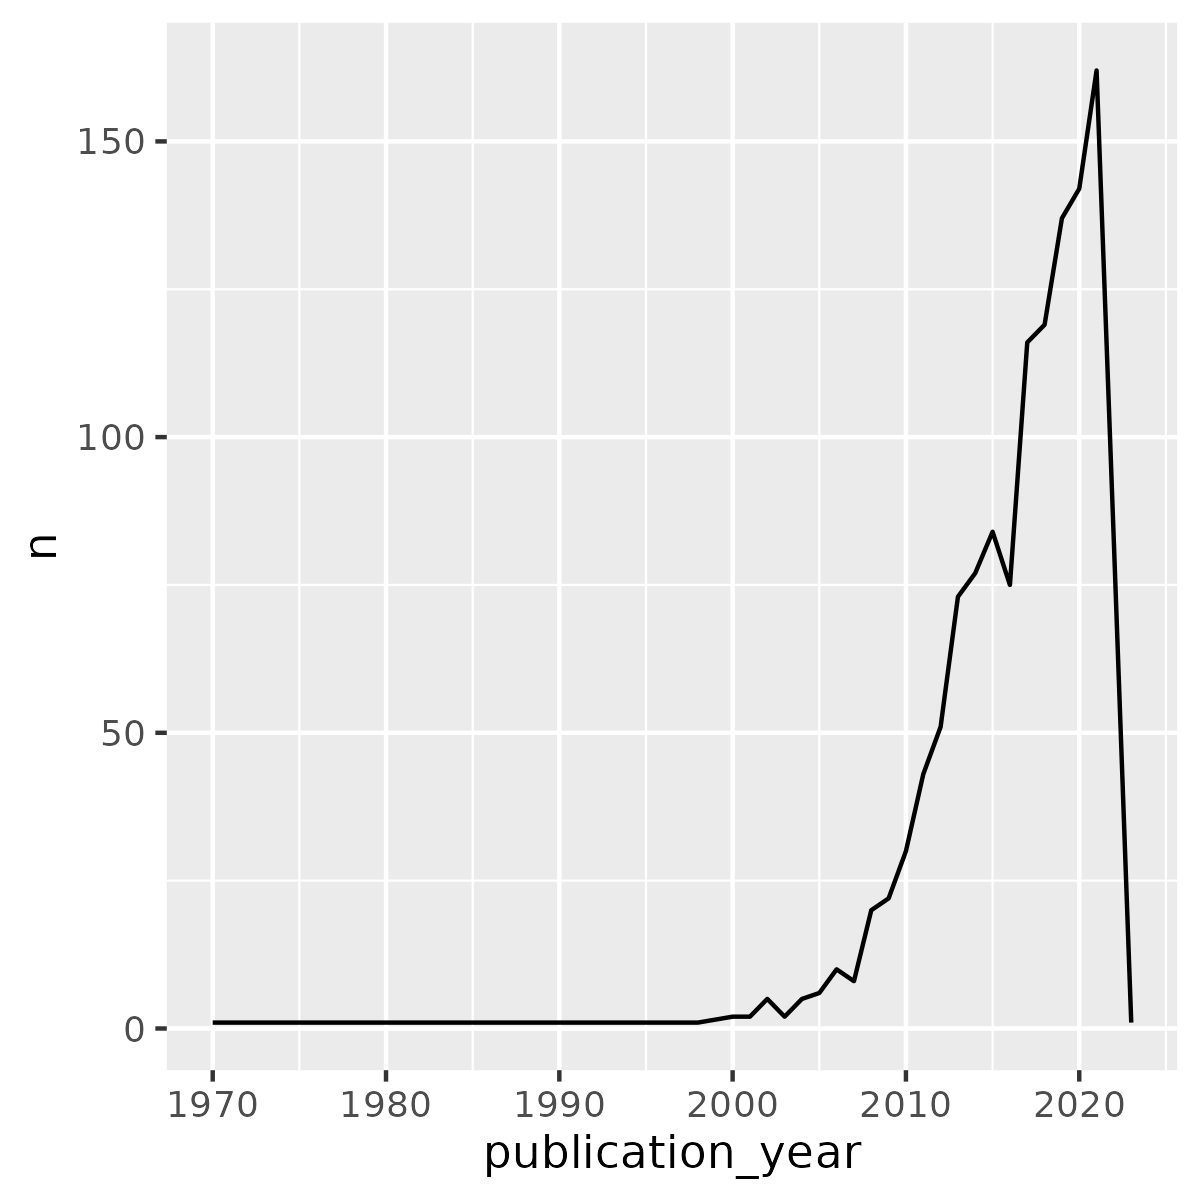
\includegraphics{plots/pubs_time_gg.png}

\end{col}

\end{cols}
\end{frame}

\begin{frame}[fragile]{A bar plot with ggplot}
\protect\hypertarget{a-bar-plot-with-ggplot}{}
\begin{cols}

\begin{col}{0.58\textwidth}

ggplot has a variety of different
\href{https://ggplot2.tidyverse.org/reference/index.html}{geoms}. Each
translates our aesthetic mapping to ink on paper in a consistent and
clearly defined way.

\medskip

\scriptsize

\begin{Shaded}
\begin{Highlighting}[]
\NormalTok{annual\_pubs }\OtherTok{\textless{}{-}}\NormalTok{ df }\SpecialCharTok{\%\textgreater{}\%} \FunctionTok{count}\NormalTok{(publication\_year) }

\FunctionTok{ggplot}\NormalTok{(annual\_pubs, }\FunctionTok{aes}\NormalTok{(publication\_year, n)) }\SpecialCharTok{+}
  \FunctionTok{geom\_col}\NormalTok{()}
\end{Highlighting}
\end{Shaded}

\begin{Shaded}
\begin{Highlighting}[]
\FunctionTok{ggsave}\NormalTok{(}\StringTok{"plots/pubs\_time\_bar\_gg.png"}\NormalTok{, }\AttributeTok{width=}\DecValTok{4}\NormalTok{, }\AttributeTok{height=}\DecValTok{4}\NormalTok{)}
\end{Highlighting}
\end{Shaded}

\end{col}

\begin{col}{0.04\textwidth}
~

\end{col}

\begin{col}{0.38\textwidth}
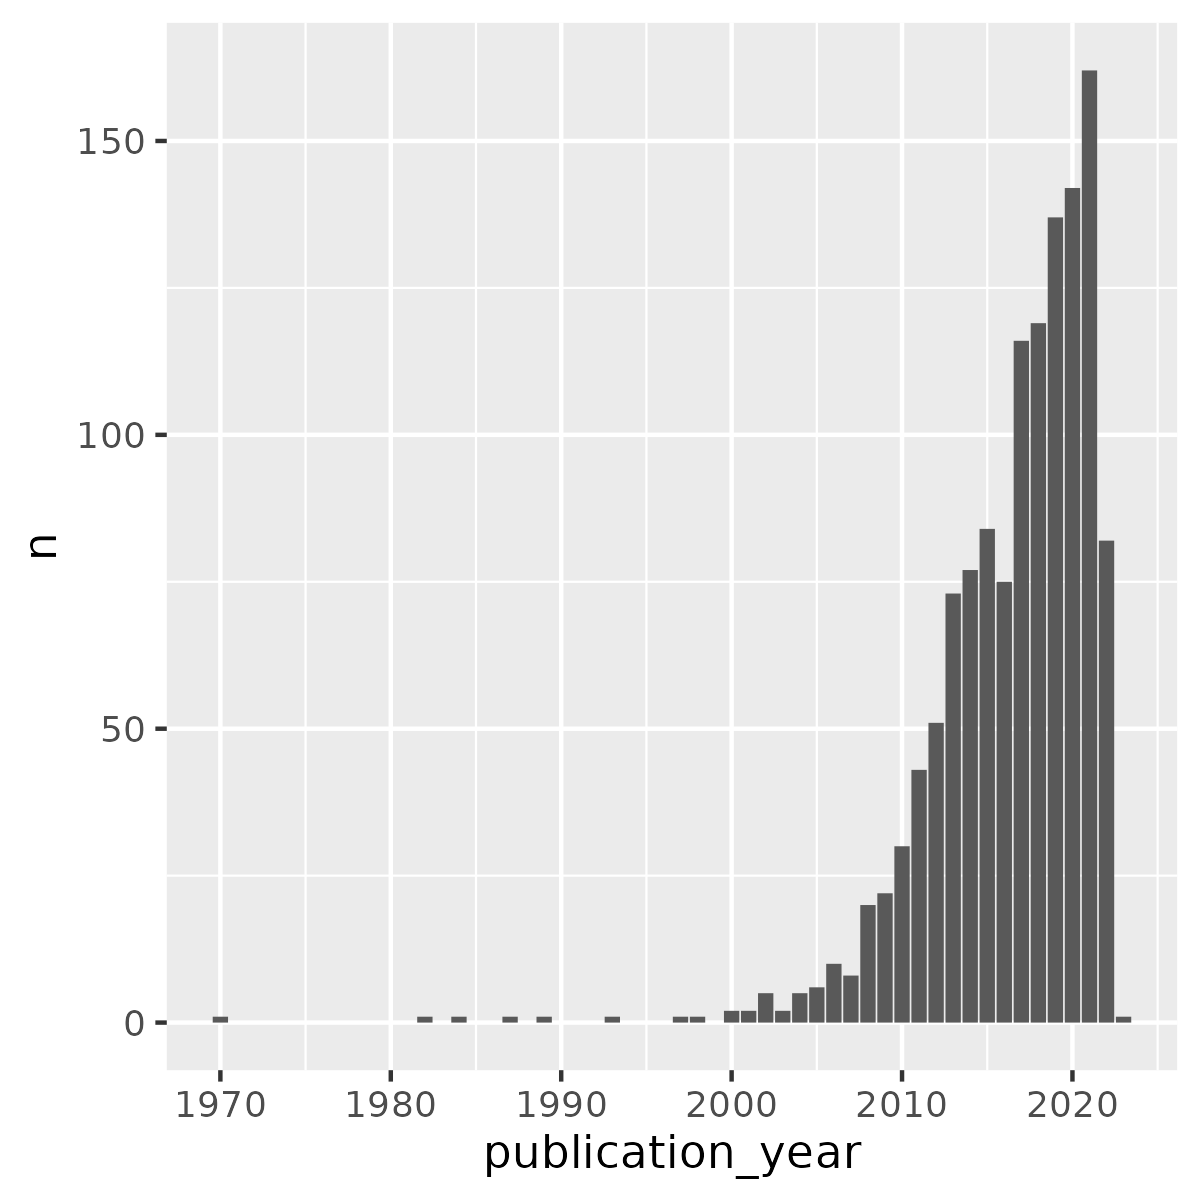
\includegraphics{plots/pubs_time_bar_gg.png}

\end{col}

\end{cols}
\end{frame}

\begin{frame}[fragile]{A scatter plot with ggplot}
\protect\hypertarget{a-scatter-plot-with-ggplot}{}
\begin{cols}

\begin{col}{0.58\textwidth}

With ggplot, we define the parameters of the plot, and then we can keep
adding ``geoms'' that inherit these parameters.

\medskip

We build up the plot bit by bit by adding more grammar. \scriptsize

\begin{Shaded}
\begin{Highlighting}[]
\NormalTok{annual\_pubs }\OtherTok{\textless{}{-}}\NormalTok{ df }\SpecialCharTok{\%\textgreater{}\%} \FunctionTok{count}\NormalTok{(publication\_year) }

\FunctionTok{ggplot}\NormalTok{(annual\_pubs, }\FunctionTok{aes}\NormalTok{(publication\_year, n)) }\SpecialCharTok{+}
  \FunctionTok{geom\_line}\NormalTok{() }\SpecialCharTok{+} 
  \FunctionTok{geom\_point}\NormalTok{() }\SpecialCharTok{+} 
  \FunctionTok{theme\_bw}\NormalTok{() }\SpecialCharTok{+}
  \FunctionTok{labs}\NormalTok{(}
    \AttributeTok{title=}\StringTok{"Publications by someone with a Hertie affiliation"}\NormalTok{, }
    \AttributeTok{x=}\StringTok{"Publication Year"}
\NormalTok{  )}
\end{Highlighting}
\end{Shaded}

\begin{Shaded}
\begin{Highlighting}[]
\FunctionTok{ggsave}\NormalTok{(}\StringTok{"plots/pubs\_time\_point\_gg.png"}\NormalTok{, }\AttributeTok{width=}\DecValTok{4}\NormalTok{, }\AttributeTok{height=}\DecValTok{4}\NormalTok{)}
\end{Highlighting}
\end{Shaded}

\end{col}

\begin{col}{0.04\textwidth}
~

\end{col}

\begin{col}{0.38\textwidth}
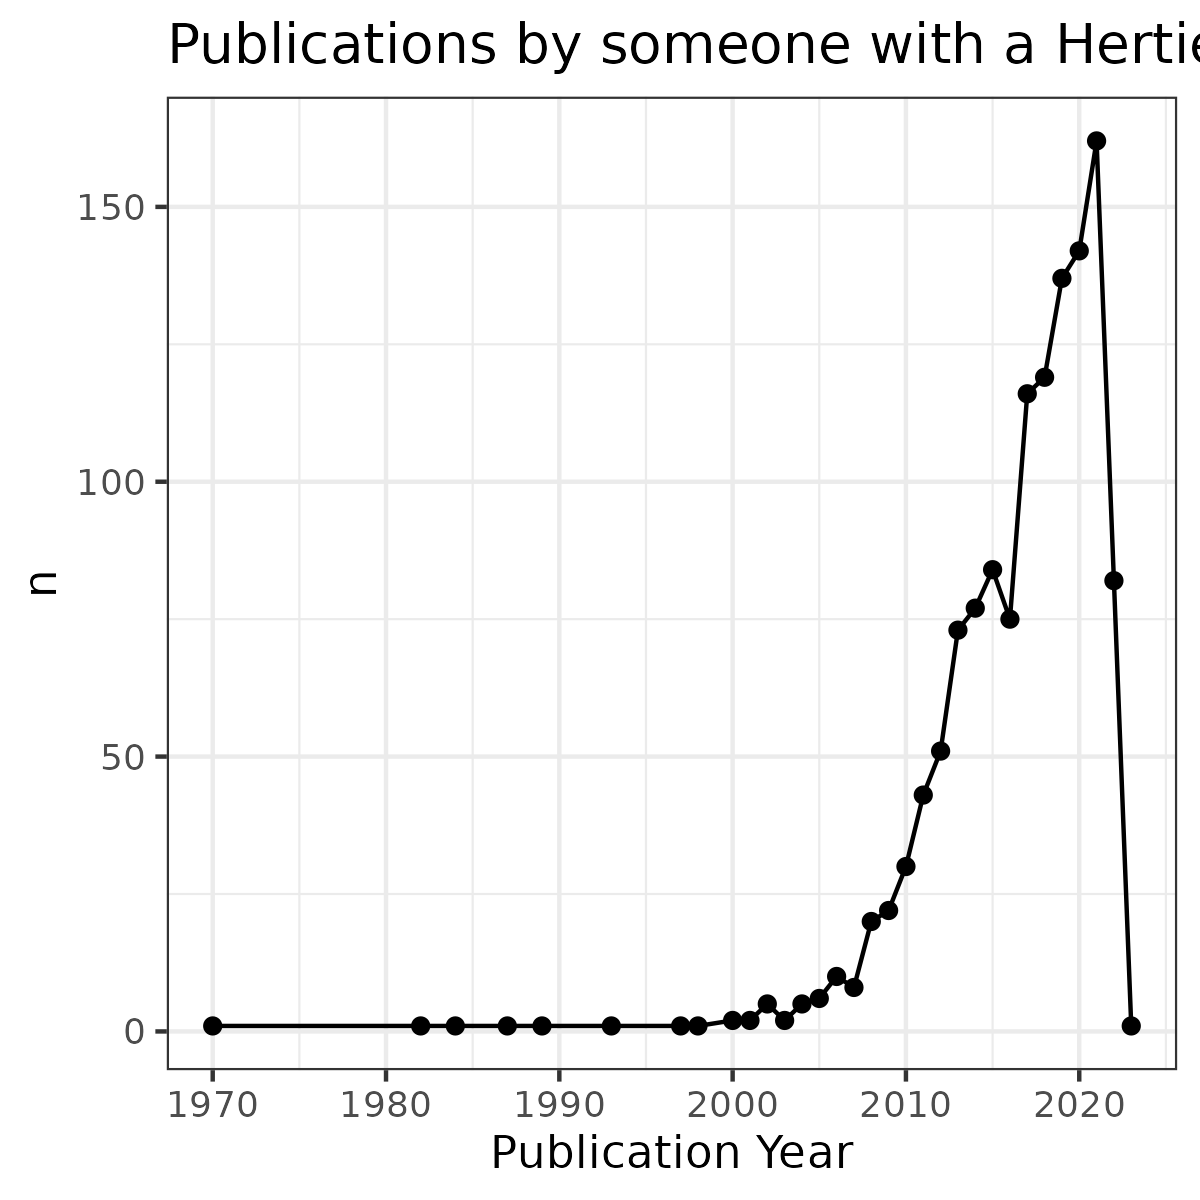
\includegraphics{plots/pubs_time_point_gg.png}

\end{col}

\end{cols}
\end{frame}

\begin{frame}[fragile]{A line plot with seaborn}
\protect\hypertarget{a-line-plot-with-seaborn}{}
\begin{cols}

\begin{col}{0.58\textwidth}

Seaborn works nicely with things in dataframes, so we need to groupby
and count, and coerce the result into a dataframe

\scriptsize

\begin{Shaded}
\begin{Highlighting}[]
\ImportTok{import}\NormalTok{ matplotlib.pyplot }\ImportTok{as}\NormalTok{ plt}
\ImportTok{import}\NormalTok{ seaborn }\ImportTok{as}\NormalTok{ sns}
\NormalTok{df }\OperatorTok{=}\NormalTok{ pd.read\_csv(}\StringTok{"data/hertie\_papers.csv"}\NormalTok{)}
\NormalTok{yps }\OperatorTok{=}\NormalTok{ (df}
\NormalTok{        .groupby([}\StringTok{"publication\_year"}\NormalTok{])[}\StringTok{"id"}\NormalTok{]}
\NormalTok{        .count()}
\NormalTok{        .to\_frame(}\StringTok{"n\_pubs"}\NormalTok{)}
\NormalTok{        .reset\_index()}
\NormalTok{      )}
\NormalTok{ax }\OperatorTok{=}\NormalTok{ sns.relplot(}
\NormalTok{  data}\OperatorTok{=}\NormalTok{yps, kind}\OperatorTok{=}\StringTok{"line"}\NormalTok{, }
\NormalTok{  x}\OperatorTok{=}\StringTok{"publication\_year"}\NormalTok{, y}\OperatorTok{=}\StringTok{"n\_pubs"}
\NormalTok{)}
\NormalTok{ax.}\BuiltInTok{set}\NormalTok{(xlabel}\OperatorTok{=}\StringTok{"Publication Year"}\NormalTok{, ylabel}\OperatorTok{=}\StringTok{"Number of publications"}\NormalTok{)}
\end{Highlighting}
\end{Shaded}

\begin{Shaded}
\begin{Highlighting}[]
\NormalTok{plt.savefig(}\StringTok{"plots/pubs\_time\_sns.png"}\NormalTok{)}
\end{Highlighting}
\end{Shaded}

\end{col}

\begin{col}{0.04\textwidth}
~

\end{col}

\begin{col}{0.38\textwidth}
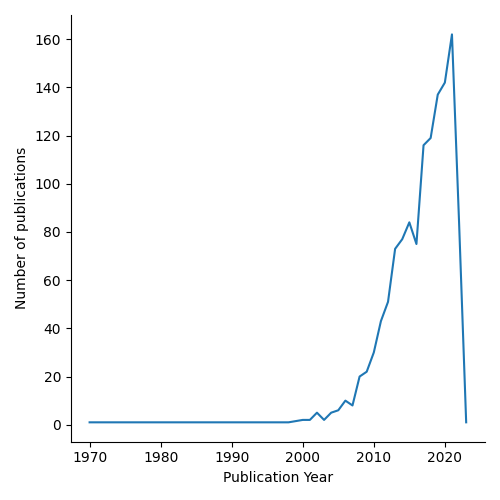
\includegraphics{plots/pubs_time_sns.png}

\end{col}

\end{cols}
\end{frame}

\begin{frame}[fragile]{A line plot with pandas}
\protect\hypertarget{a-line-plot-with-pandas}{}
\begin{cols}

\begin{col}{0.58\textwidth}

Pandas can already produce a lot of the plots we want

\scriptsize

\begin{Shaded}
\begin{Highlighting}[]
\ImportTok{import}\NormalTok{ matplotlib.pyplot }\ImportTok{as}\NormalTok{ plt}
\ImportTok{import}\NormalTok{ seaborn }\ImportTok{as}\NormalTok{ sns}
\NormalTok{fig, ax }\OperatorTok{=}\NormalTok{ plt.subplots(figsize}\OperatorTok{=}\NormalTok{(}\DecValTok{4}\NormalTok{,}\DecValTok{4}\NormalTok{))}
\NormalTok{df.groupby([}\StringTok{"publication\_year"}\NormalTok{])[}\StringTok{"id"}\NormalTok{].count().plot(ax}\OperatorTok{=}\NormalTok{ax)}
\NormalTok{ax.set\_xlabel(}\StringTok{"Publication Year"}\NormalTok{)}
\NormalTok{ax.set\_ylabel(}\StringTok{"Number of Publications"}\NormalTok{)}
\NormalTok{ax.set\_title(}\StringTok{"Publications by someone with a Hertie affiliation"}\NormalTok{)}
\NormalTok{plt.savefig(}\StringTok{"plots/pubs\_time\_pd.png"}\NormalTok{)}
\end{Highlighting}
\end{Shaded}

\end{col}

\begin{col}{0.04\textwidth}
~

\end{col}

\begin{col}{0.38\textwidth}
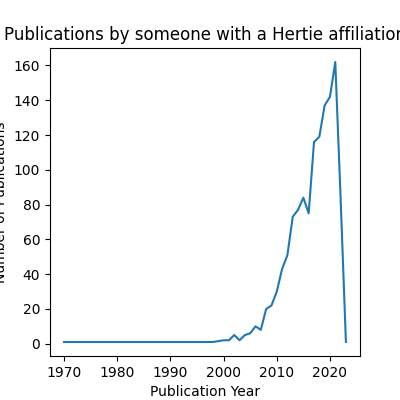
\includegraphics{plots/pubs_time_pd.png}

\end{col}

\end{cols}
\end{frame}

\begin{frame}[fragile]{A bar plot with seaborn}
\protect\hypertarget{a-bar-plot-with-seaborn}{}
\begin{cols}

\begin{col}{0.58\textwidth}

Seaborn is also ``opinionated'' and makes strong assumptions about what
you want to do. According to seaborn, if you are making a bar plot, then
one of your variables is likely categorical and it will plot it
accordingly.

\medskip

\scriptsize

\begin{Shaded}
\begin{Highlighting}[]
\ImportTok{import}\NormalTok{ matplotlib.pyplot }\ImportTok{as}\NormalTok{ plt}
\ImportTok{import}\NormalTok{ seaborn }\ImportTok{as}\NormalTok{ sns}
\NormalTok{df }\OperatorTok{=}\NormalTok{ pd.read\_csv(}\StringTok{"data/hertie\_papers.csv"}\NormalTok{)}
\NormalTok{yps }\OperatorTok{=}\NormalTok{ (df}
\NormalTok{        .groupby([}\StringTok{"publication\_year"}\NormalTok{])[}\StringTok{"id"}\NormalTok{]}
\NormalTok{        .count()}
\NormalTok{        .to\_frame(}\StringTok{"n\_pubs"}\NormalTok{)}
\NormalTok{        .reset\_index()}
\NormalTok{      )}
\NormalTok{ax }\OperatorTok{=}\NormalTok{ sns.barplot(data}\OperatorTok{=}\NormalTok{yps, x}\OperatorTok{=}\StringTok{"publication\_year"}\NormalTok{, y}\OperatorTok{=}\StringTok{"n\_pubs"}\NormalTok{)}
\NormalTok{ax.}\BuiltInTok{set}\NormalTok{(xlabel}\OperatorTok{=}\StringTok{"Publication Year"}\NormalTok{, ylabel}\OperatorTok{=}\StringTok{"Number of publications"}\NormalTok{)}
\NormalTok{plt.savefig(}\StringTok{"plots/pubs\_time\_bar\_sns.png"}\NormalTok{)}
\end{Highlighting}
\end{Shaded}

\end{col}

\begin{col}{0.04\textwidth}
~

\end{col}

\begin{col}{0.38\textwidth}
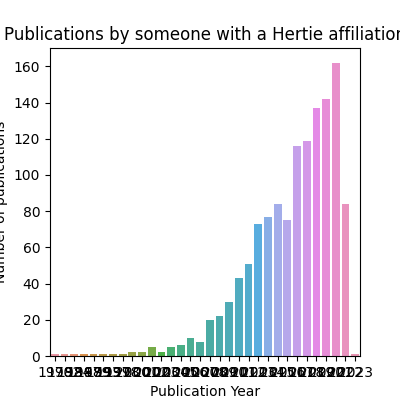
\includegraphics{plots/pubs_time_bar_sns.png}

\end{col}

\end{cols}
\end{frame}

\begin{frame}[fragile]{A bar plot with matplotlib}
\protect\hypertarget{a-bar-plot-with-matplotlib}{}
\begin{cols}

\begin{col}{0.58\textwidth}

Matplotlib is sometimes the simplest option for simple plots.

\medskip

\scriptsize

\begin{Shaded}
\begin{Highlighting}[]
\ImportTok{import}\NormalTok{ matplotlib.pyplot }\ImportTok{as}\NormalTok{ plt}
\ImportTok{import}\NormalTok{ seaborn }\ImportTok{as}\NormalTok{ sns}
\NormalTok{df }\OperatorTok{=}\NormalTok{ pd.read\_csv(}\StringTok{"data/hertie\_papers.csv"}\NormalTok{)}
\NormalTok{yps }\OperatorTok{=}\NormalTok{ (df}
\NormalTok{        .groupby([}\StringTok{"publication\_year"}\NormalTok{])[}\StringTok{"id"}\NormalTok{]}
\NormalTok{        .count()}
\NormalTok{        .to\_frame(}\StringTok{"n\_pubs"}\NormalTok{)}
\NormalTok{        .reset\_index()}
\NormalTok{      )}
\NormalTok{fig, ax }\OperatorTok{=}\NormalTok{ plt.subplots(figsize}\OperatorTok{=}\NormalTok{(}\DecValTok{4}\NormalTok{,}\DecValTok{4}\NormalTok{))}
\NormalTok{ax.bar(yps[}\StringTok{"publication\_year"}\NormalTok{], yps[}\StringTok{"n\_pubs"}\NormalTok{])}
\end{Highlighting}
\end{Shaded}

\begin{Shaded}
\begin{Highlighting}[]
\NormalTok{ax.set\_xlabel(}\StringTok{"Publication Year"}\NormalTok{)}
\NormalTok{ax.set\_ylabel(}\StringTok{"Number of Publications"}\NormalTok{)}
\NormalTok{ax.set\_title(}\StringTok{"Publications by someone with a Hertie affiliation"}\NormalTok{)}
\NormalTok{plt.savefig(}\StringTok{"plots/pubs\_time\_bar\_mpl.png"}\NormalTok{)}
\end{Highlighting}
\end{Shaded}

\end{col}

\begin{col}{0.04\textwidth}
~

\end{col}

\begin{col}{0.38\textwidth}
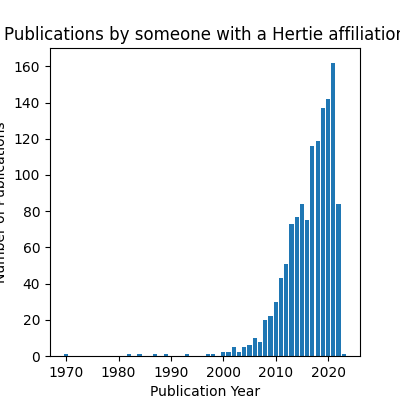
\includegraphics{plots/pubs_time_bar_mpl.png}

\end{col}

\end{cols}
\end{frame}

\begin{frame}[fragile]{Exercise}
\protect\hypertarget{exercise}{}
Load the authorship data in \texttt{data/author\_df.csv} and make a
horizontal bar plot showing the 10 authors who have published the most
papers \emph{with Hertie affiliations}. In R you may need the functions
\texttt{filter()}, \texttt{count()}, \texttt{arrange()}, and
\texttt{head()/tail()}. In python you will need to filter data
\texttt{df{[}df{[}"x"{]}=="y"{]}}, and to use the
\texttt{sort\_values()} as well as \texttt{head()/tail()}
\end{frame}

\hypertarget{plotting-text-data}{%
\section{Plotting text data}\label{plotting-text-data}}

\begin{frame}{What text data can we plot}
\protect\hypertarget{what-text-data-can-we-plot}{}
\begin{itemize}
\tightlist
\item
  Frequencies of features
\item
  frequencies of features in subgroups or over time
\item
  relationships between features
\item
  relationships between features and text/author variables
\end{itemize}
\end{frame}

\begin{frame}[fragile]{Back to our document feature matrix}
\protect\hypertarget{back-to-our-document-feature-matrix}{}
Let's create a document feature matrix from our list of abstracts

\scriptsize

\begin{Shaded}
\begin{Highlighting}[]
\FunctionTok{library}\NormalTok{(quanteda)}
\NormalTok{df }\OtherTok{\textless{}{-}}\NormalTok{ df }\SpecialCharTok{\%\textgreater{}\%} \FunctionTok{filter}\NormalTok{(}\SpecialCharTok{!}\FunctionTok{is.na}\NormalTok{(abstract))}
\NormalTok{dfmat }\OtherTok{\textless{}{-}}\NormalTok{ df}\SpecialCharTok{$}\NormalTok{abstract }\SpecialCharTok{\%\textgreater{}\%}
  \FunctionTok{tokens}\NormalTok{(}\AttributeTok{remove\_punc=}\ConstantTok{TRUE}\NormalTok{) }\SpecialCharTok{\%\textgreater{}\%}
  \FunctionTok{tokens\_remove}\NormalTok{(}\AttributeTok{pattern=}\FunctionTok{stopwords}\NormalTok{(}\StringTok{"en"}\NormalTok{)) }\SpecialCharTok{\%\textgreater{}\%}
  \FunctionTok{tokens\_wordstem}\NormalTok{(}\StringTok{"english"}\NormalTok{) }\SpecialCharTok{\%\textgreater{}\%}
  \FunctionTok{dfm}\NormalTok{()}
\NormalTok{dfmat}
\end{Highlighting}
\end{Shaded}

\begin{verbatim}
## Document-feature matrix of: 1,112 documents, 12,035 features (99.41% sparse) and 0 docvars.
##        features
## docs    > 50 chanc limit warm 2 ° c recent scenario
##   text1 1  1     1     2    1 1 1 1      1        1
##   text2 0  0     0     0    0 0 0 0      0        0
##   text3 0  0     0     1    0 0 0 0      1        0
##   text4 0  0     0     1    0 0 0 0      0        0
##   text5 0  0     0     0    0 0 0 0      0        0
##   text6 0  0     0     0    0 0 0 0      0        0
## [ reached max_ndoc ... 1,106 more documents, reached max_nfeat ... 12,025 more features ]
\end{verbatim}

\begin{Shaded}
\begin{Highlighting}[]
\ImportTok{from}\NormalTok{ sklearn.feature\_extraction.text }\ImportTok{import}\NormalTok{ CountVectorizer, TfidfVectorizer}
\NormalTok{vectorizer }\OperatorTok{=}\NormalTok{ CountVectorizer(stop\_words}\OperatorTok{=}\StringTok{"english"}\NormalTok{)}
\NormalTok{df }\OperatorTok{=}\NormalTok{ df[pd.notna(df[}\StringTok{"abstract"}\NormalTok{])].reset\_index(drop}\OperatorTok{=}\VariableTok{True}\NormalTok{)}
\NormalTok{dfm }\OperatorTok{=}\NormalTok{ vectorizer.fit\_transform(df[}\StringTok{"abstract"}\NormalTok{])}
\NormalTok{dfm}
\end{Highlighting}
\end{Shaded}

\begin{verbatim}
## <1115x15084 sparse matrix of type '<class 'numpy.int64'>'
##  with 78193 stored elements in Compressed Sparse Row format>
\end{verbatim}
\end{frame}

\begin{frame}[fragile]{Most common features}
\protect\hypertarget{most-common-features}{}
\begin{cols}

\begin{col}{0.58\textwidth}

\texttt{quanteda.textstats::textstat\_frequency()} gives us the
frequency of each term in the corpus. \medskip 

\scriptsize

\begin{Shaded}
\begin{Highlighting}[]
\FunctionTok{library}\NormalTok{(quanteda.textstats)}
\NormalTok{tfreq }\OtherTok{\textless{}{-}}\NormalTok{ dfmat }\SpecialCharTok{\%\textgreater{}\%} \FunctionTok{textstat\_frequency}\NormalTok{() }\SpecialCharTok{\%\textgreater{}\%} \FunctionTok{head}\NormalTok{(}\DecValTok{20}\NormalTok{)}
\NormalTok{tfreq}\SpecialCharTok{$}\NormalTok{feature }\OtherTok{\textless{}{-}} \FunctionTok{factor}\NormalTok{(tfreq}\SpecialCharTok{$}\NormalTok{feature, }\AttributeTok{levels=}\NormalTok{tfreq}\SpecialCharTok{$}\NormalTok{feature)}
\FunctionTok{ggplot}\NormalTok{(tfreq, }\FunctionTok{aes}\NormalTok{(}\AttributeTok{x=}\NormalTok{frequency, }\AttributeTok{y=}\NormalTok{feature)) }\SpecialCharTok{+}
  \FunctionTok{geom\_col}\NormalTok{()}
\end{Highlighting}
\end{Shaded}

\begin{Shaded}
\begin{Highlighting}[]
\FunctionTok{ggsave}\NormalTok{(}\StringTok{"plots/top\_terms\_gg.png"}\NormalTok{, }\AttributeTok{width=}\DecValTok{4}\NormalTok{, }\AttributeTok{height=}\DecValTok{4}\NormalTok{)}
\end{Highlighting}
\end{Shaded}

\end{col}

\begin{col}{0.04\textwidth}
~

\end{col}

\begin{col}{0.38\textwidth}
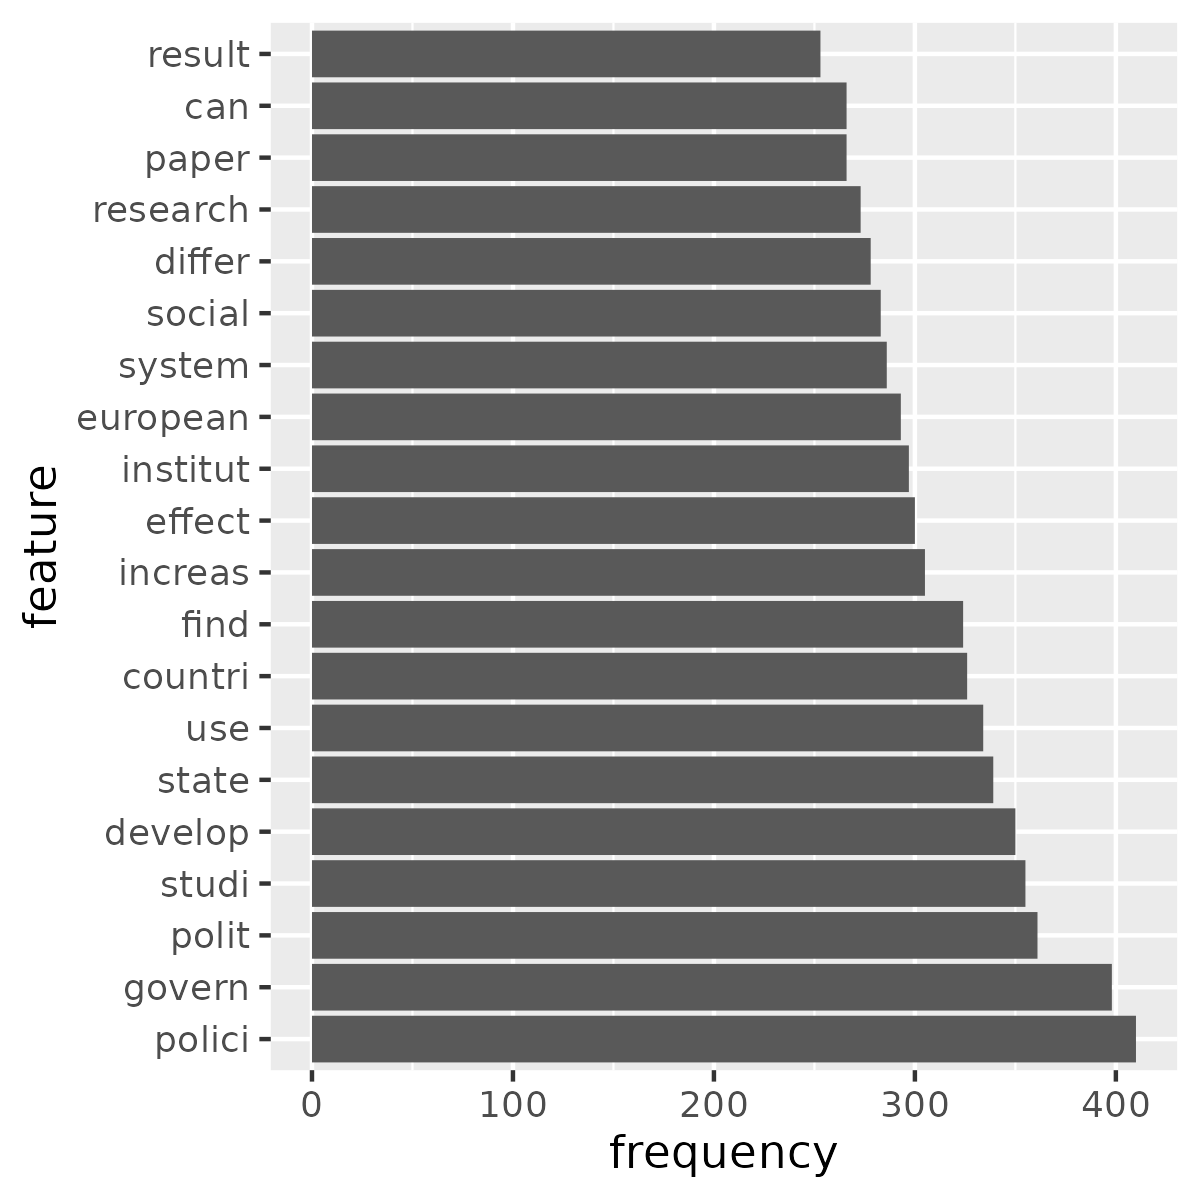
\includegraphics{plots/top_terms_gg.png}

\end{col}

\end{cols}
\end{frame}

\begin{frame}[fragile]{Common features in subgroups}
\protect\hypertarget{common-features-in-subgroups}{}
\begin{cols}

\begin{col}{0.58\textwidth}

We can also get the frequency of features per subgroup \medskip 

\scriptsize

\begin{Shaded}
\begin{Highlighting}[]
\NormalTok{ytfreq }\OtherTok{\textless{}{-}}\NormalTok{ dfmat }\SpecialCharTok{\%\textgreater{}\%} 
  \FunctionTok{textstat\_frequency}\NormalTok{(}\AttributeTok{groups=}\NormalTok{df}\SpecialCharTok{$}\NormalTok{publication\_year) }
\NormalTok{ytfreq}\SpecialCharTok{$}\NormalTok{group }\OtherTok{\textless{}{-}} \FunctionTok{as.numeric}\NormalTok{(ytfreq}\SpecialCharTok{$}\NormalTok{group)}
\NormalTok{interesting\_features }\OtherTok{\textless{}{-}}\NormalTok{ ytfreq }\SpecialCharTok{\%\textgreater{}\%}
  \FunctionTok{filter}\NormalTok{(feature }\SpecialCharTok{\%in\%} \FunctionTok{c}\NormalTok{(}\StringTok{"european"}\NormalTok{,}\StringTok{"climat"}\NormalTok{))}

\FunctionTok{ggplot}\NormalTok{(}
\NormalTok{  interesting\_features, }
  \FunctionTok{aes}\NormalTok{(}\AttributeTok{x=}\NormalTok{group, }\AttributeTok{y=}\NormalTok{frequency, }\AttributeTok{colour=}\NormalTok{feature)}
\NormalTok{) }\SpecialCharTok{+}
  \FunctionTok{geom\_point}\NormalTok{() }\SpecialCharTok{+}
  \FunctionTok{geom\_line}\NormalTok{() }\SpecialCharTok{+} 
  \FunctionTok{theme\_bw}\NormalTok{()}
\end{Highlighting}
\end{Shaded}

\begin{Shaded}
\begin{Highlighting}[]
\FunctionTok{ggsave}\NormalTok{(}\StringTok{"plots/top\_terms\_time.png"}\NormalTok{, }\AttributeTok{width=}\DecValTok{4}\NormalTok{, }\AttributeTok{height=}\DecValTok{4}\NormalTok{)}
\end{Highlighting}
\end{Shaded}

\end{col}

\begin{col}{0.04\textwidth}
~

\end{col}

\begin{col}{0.38\textwidth}
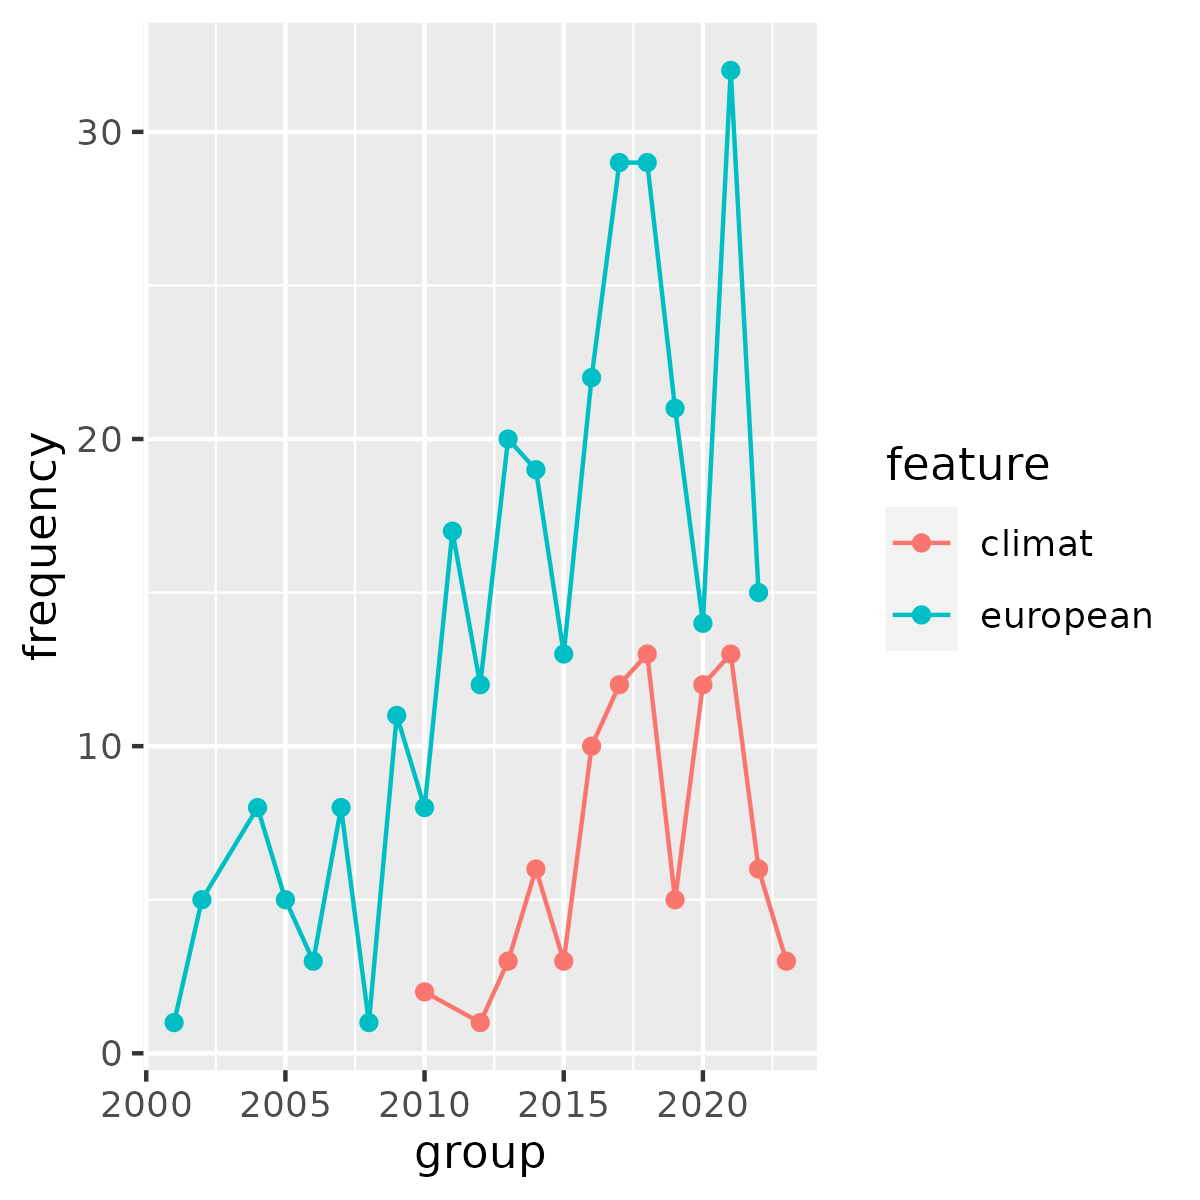
\includegraphics{plots/top_terms_time_gg.png}

\end{col}

\end{cols}
\end{frame}

\begin{frame}[fragile]{Most common features in Python}
\protect\hypertarget{most-common-features-in-python}{}
\begin{cols}

\begin{col}{0.58\textwidth}

In pandas we can make a dataframe of the sum of each column and the
feature names \medskip 

\scriptsize

\begin{Shaded}
\begin{Highlighting}[]
\NormalTok{counts }\OperatorTok{=}\NormalTok{ dfm.}\BuiltInTok{sum}\NormalTok{(axis}\OperatorTok{=}\DecValTok{0}\NormalTok{).A1}
\NormalTok{tidy\_dfm }\OperatorTok{=}\NormalTok{ pd.DataFrame(\{}
    \StringTok{"count"}\NormalTok{: counts, }
    \StringTok{"feature"}\NormalTok{: vectorizer.get\_feature\_names\_out()}
\NormalTok{\}).sort\_values(}\StringTok{"count"}\NormalTok{,ascending}\OperatorTok{=}\VariableTok{False}\NormalTok{).reset\_index(drop}\OperatorTok{=}\VariableTok{True}\NormalTok{)}

\NormalTok{fig, ax }\OperatorTok{=}\NormalTok{ plt.subplots(figsize}\OperatorTok{=}\NormalTok{(}\DecValTok{4}\NormalTok{,}\DecValTok{4}\NormalTok{))}
\NormalTok{sns.barplot(data}\OperatorTok{=}\NormalTok{tidy\_dfm.head(), x}\OperatorTok{=}\StringTok{"count"}\NormalTok{, y}\OperatorTok{=}\StringTok{"feature"}\NormalTok{, color}\OperatorTok{=}\StringTok{"grey"}\NormalTok{)}

\NormalTok{plt.savefig(}\StringTok{"plots/top\_terms\_sns.png"}\NormalTok{)}
\end{Highlighting}
\end{Shaded}

\end{col}

\begin{col}{0.04\textwidth}
~

\end{col}

\begin{col}{0.38\textwidth}
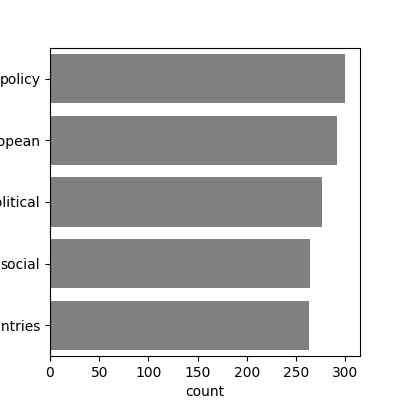
\includegraphics{plots/top_terms_sns.png}

\end{col}

\end{cols}
\end{frame}

\begin{frame}[fragile]{Common features in subgroups in Python}
\protect\hypertarget{common-features-in-subgroups-in-python}{}
\begin{cols}

\begin{col}{0.58\textwidth}

Summing the features per subgroup in Python simply requires some
low-level arithmetic and indexing \medskip 

\scriptsize

\begin{Shaded}
\begin{Highlighting}[]
\NormalTok{tidy\_dfm }\OperatorTok{=}\NormalTok{ pd.DataFrame()}
\NormalTok{features }\OperatorTok{=}\NormalTok{ vectorizer.get\_feature\_names\_out()}
\ControlFlowTok{for}\NormalTok{ name, group }\KeywordTok{in}\NormalTok{ df.groupby(}\StringTok{"publication\_year"}\NormalTok{):}
\NormalTok{    counts }\OperatorTok{=}\NormalTok{ dfm[group.index,:].}\BuiltInTok{sum}\NormalTok{(axis}\OperatorTok{=}\DecValTok{0}\NormalTok{).A1}
\NormalTok{    group\_df }\OperatorTok{=}\NormalTok{ pd.DataFrame(\{}
        \StringTok{"count"}\NormalTok{: counts,}
        \StringTok{"feature"}\NormalTok{: features,}
        \StringTok{"group"}\NormalTok{: name}
\NormalTok{    \})}
\NormalTok{    tidy\_dfm }\OperatorTok{=}\NormalTok{ pd.concat([}
\NormalTok{      tidy\_dfm, }
\NormalTok{      group\_df[group\_df[}\StringTok{"count"}\NormalTok{]}\OperatorTok{!=}\DecValTok{0}\NormalTok{]}
\NormalTok{    ]).reset\_index(drop}\OperatorTok{=}\VariableTok{True}\NormalTok{)}

\NormalTok{interesting\_features }\OperatorTok{=}\NormalTok{ tidy\_dfm[}
\NormalTok{  tidy\_dfm[}\StringTok{"feature"}\NormalTok{].isin([}\StringTok{"climate"}\NormalTok{,}\StringTok{"european"}\NormalTok{])}
\NormalTok{]}
\NormalTok{sns.relplot(}
\NormalTok{  data}\OperatorTok{=}\NormalTok{interesting\_features, x}\OperatorTok{=}\StringTok{"group"}\NormalTok{, y}\OperatorTok{=}\StringTok{"count"}\NormalTok{, }
\NormalTok{  hue}\OperatorTok{=}\StringTok{"feature"}\NormalTok{, kind}\OperatorTok{=}\StringTok{"line"}
\NormalTok{)}
\end{Highlighting}
\end{Shaded}

\begin{Shaded}
\begin{Highlighting}[]
\NormalTok{plt.savefig(}\StringTok{"plots/top\_terms\_time\_sns.png"}\NormalTok{)}
\end{Highlighting}
\end{Shaded}

\end{col}

\begin{col}{0.04\textwidth}
~

\end{col}

\begin{col}{0.38\textwidth}
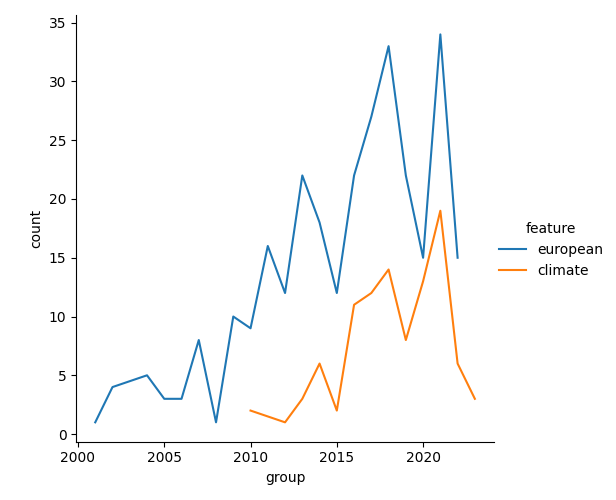
\includegraphics{plots/top_terms_time_sns.png}

\end{col}

\end{cols}
\end{frame}

\begin{frame}[fragile]{Comparing subgroups}
\protect\hypertarget{comparing-subgroups}{}
\begin{cols}

\begin{col}{0.58\textwidth}

If we want to compare two subgroups directly, we might plot one against
the other \medskip 

\scriptsize

\begin{Shaded}
\begin{Highlighting}[]
\FunctionTok{library}\NormalTok{(quanteda.textstats)}
\NormalTok{df}\SpecialCharTok{$}\NormalTok{era }\OtherTok{\textless{}{-}} \FunctionTok{ifelse}\NormalTok{(df}\SpecialCharTok{$}\NormalTok{publication\_year}\SpecialCharTok{\textless{}}\DecValTok{2017}\NormalTok{, }\StringTok{"Pre"}\NormalTok{, }\StringTok{"Post"}\NormalTok{)}

\NormalTok{ytfreq }\OtherTok{\textless{}{-}}\NormalTok{ dfmat }\SpecialCharTok{\%\textgreater{}\%} \FunctionTok{textstat\_frequency}\NormalTok{(}\AttributeTok{groups=}\NormalTok{df}\SpecialCharTok{$}\NormalTok{era) }\SpecialCharTok{\%\textgreater{}\%}
  \FunctionTok{pivot\_wider}\NormalTok{(}\AttributeTok{id\_cols=}\NormalTok{feature, }\AttributeTok{names\_from=}\NormalTok{group, }\AttributeTok{values\_from=}\NormalTok{frequency)}

\FunctionTok{ggplot}\NormalTok{(ytfreq, }\FunctionTok{aes}\NormalTok{(}\AttributeTok{x=}\NormalTok{Post, }\AttributeTok{y=}\NormalTok{Pre)) }\SpecialCharTok{+}
  \FunctionTok{geom\_point}\NormalTok{() }\SpecialCharTok{+} 
  \FunctionTok{coord\_fixed}\NormalTok{()}
\end{Highlighting}
\end{Shaded}

\begin{verbatim}
## Warning: Removed 8427 rows containing missing values (geom_point).
\end{verbatim}

\begin{Shaded}
\begin{Highlighting}[]
\FunctionTok{ggsave}\NormalTok{(}\StringTok{"plots/scattertext\_gg.png"}\NormalTok{, }\AttributeTok{width=}\DecValTok{4}\NormalTok{, }\AttributeTok{height=}\DecValTok{4}\NormalTok{)}
\end{Highlighting}
\end{Shaded}

\begin{verbatim}
## Warning: Removed 8427 rows containing missing values (geom_point).
\end{verbatim}

\end{col}

\begin{col}{0.04\textwidth}
~

\end{col}

\begin{col}{0.38\textwidth}
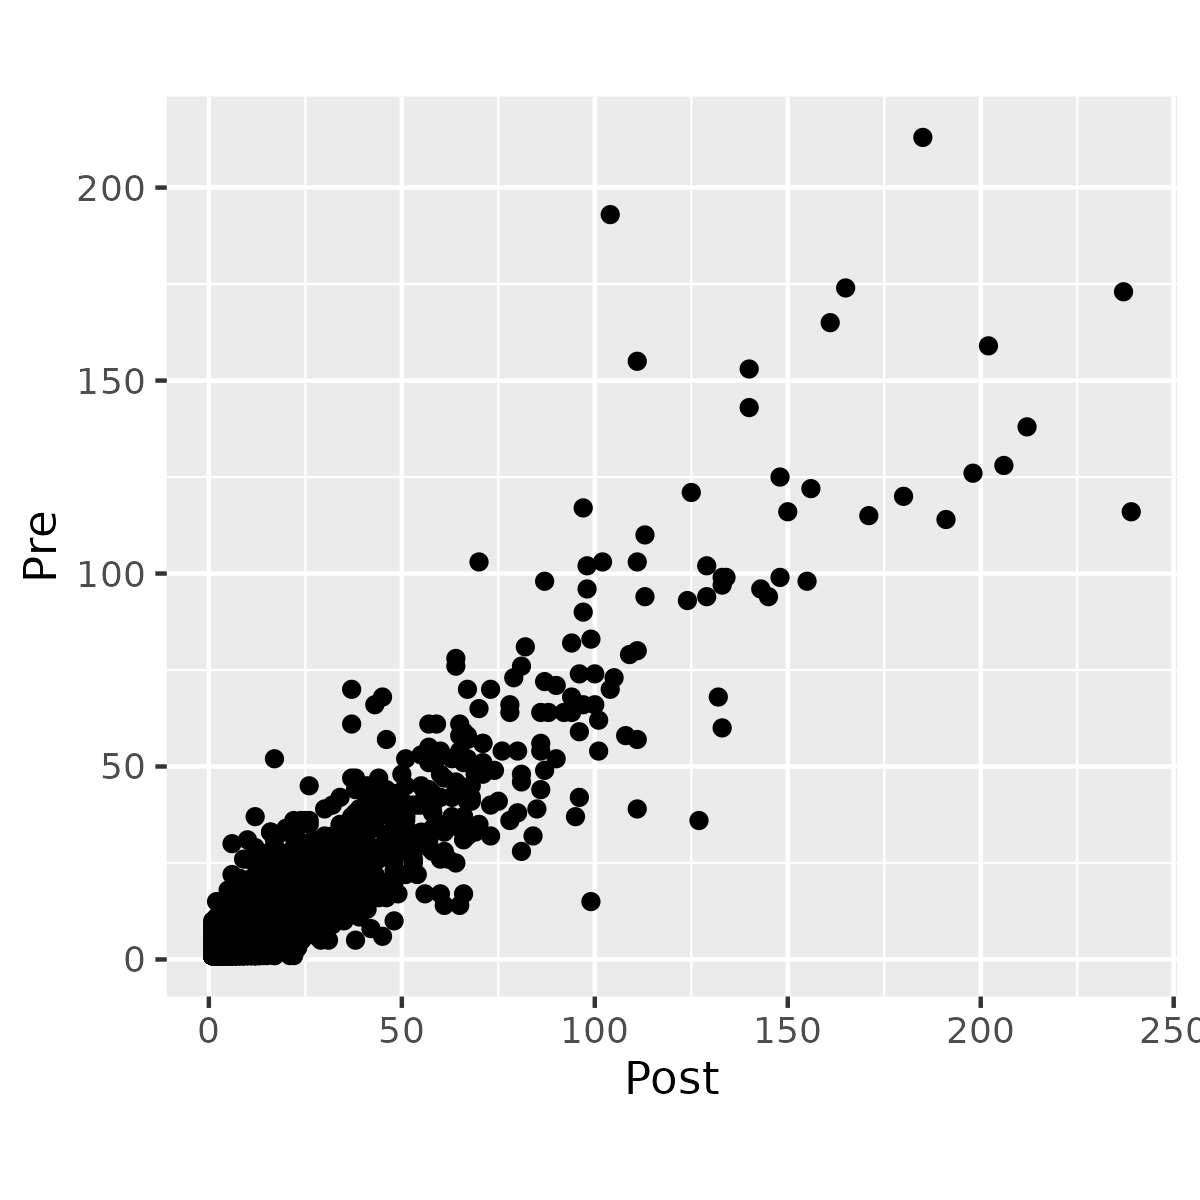
\includegraphics{plots/scattertext_gg.png}

\end{col}

\end{cols}
\end{frame}

\begin{frame}[fragile]{Long vs wide data}
\protect\hypertarget{long-vs-wide-data}{}
We often need to rely on the \texttt{tidyr::pivot\_wider()} and
\texttt{tidyr::pivot\_longer()} functions (formerly \texttt{spread()}
and \texttt{gather()}) to get data into the format we need.

\tiny

\begin{cols}

\begin{col}{0.32\textwidth}

\begin{Shaded}
\begin{Highlighting}[]
\NormalTok{dfmat }\SpecialCharTok{\%\textgreater{}\%} \FunctionTok{textstat\_frequency}\NormalTok{(}\AttributeTok{groups=}\NormalTok{df}\SpecialCharTok{$}\NormalTok{era) }\SpecialCharTok{\%\textgreater{}\%}
  \FunctionTok{head}\NormalTok{()}
\end{Highlighting}
\end{Shaded}

\begin{verbatim}
##   feature frequency rank docfreq group
## 1   studi       239    1     176  Post
## 2  polici       237    2     165  Post
## 3 develop       212    3     149  Post
## 4     use       206    4     172  Post
## 5   polit       202    5     162  Post
## 6    find       198    6     177  Post
\end{verbatim}

\end{col}

\begin{col}{0.03\textwidth}
~

\end{col}

\begin{col}{0.32\textwidth}

\begin{Shaded}
\begin{Highlighting}[]
\NormalTok{dfmat }\SpecialCharTok{\%\textgreater{}\%} \FunctionTok{textstat\_frequency}\NormalTok{(}\AttributeTok{groups=}\NormalTok{df}\SpecialCharTok{$}\NormalTok{era) }\SpecialCharTok{\%\textgreater{}\%}
  \FunctionTok{pivot\_wider}\NormalTok{(}\AttributeTok{id\_cols=}\NormalTok{feature, }\AttributeTok{names\_from=}\NormalTok{group, }\AttributeTok{values\_from=}\NormalTok{frequency) }\SpecialCharTok{\%\textgreater{}\%}
  \FunctionTok{head}\NormalTok{()}
\end{Highlighting}
\end{Shaded}

\begin{verbatim}
## # A tibble: 6 x 3
##   feature  Post   Pre
##   <chr>   <dbl> <dbl>
## 1 studi     239   116
## 2 polici    237   173
## 3 develop   212   138
## 4 use       206   128
## 5 polit     202   159
## 6 find      198   126
\end{verbatim}

\end{col}

\begin{col}{0.03\textwidth}
~

\end{col}

\begin{col}{0.32\textwidth}

\begin{Shaded}
\begin{Highlighting}[]
\NormalTok{dfmat }\SpecialCharTok{\%\textgreater{}\%} \FunctionTok{textstat\_frequency}\NormalTok{(}\AttributeTok{groups=}\NormalTok{df}\SpecialCharTok{$}\NormalTok{era) }\SpecialCharTok{\%\textgreater{}\%}
  \FunctionTok{pivot\_wider}\NormalTok{(}\AttributeTok{id\_cols=}\NormalTok{feature, }\AttributeTok{names\_from=}\NormalTok{group, }\AttributeTok{values\_from=}\NormalTok{frequency) }\SpecialCharTok{\%\textgreater{}\%}
  \FunctionTok{pivot\_longer}\NormalTok{(}\AttributeTok{cols=}\NormalTok{Post}\SpecialCharTok{:}\NormalTok{Pre, }\AttributeTok{names\_to=}\StringTok{"group"}\NormalTok{) }\SpecialCharTok{\%\textgreater{}\%}
  \FunctionTok{head}\NormalTok{()}
\end{Highlighting}
\end{Shaded}

\begin{verbatim}
## # A tibble: 6 x 3
##   feature group value
##   <chr>   <chr> <dbl>
## 1 studi   Post    239
## 2 studi   Pre     116
## 3 polici  Post    237
## 4 polici  Pre     173
## 5 develop Post    212
## 6 develop Pre     138
\end{verbatim}

\end{col}

\end{cols}
\end{frame}

\begin{frame}[fragile]{Comparing subgroups}
\protect\hypertarget{comparing-subgroups-1}{}
\begin{cols}

\begin{col}{0.58\textwidth}

In Pandas the functions we need to switch between wide and long data are
\texttt{pivot\_table()} and \texttt{melt()} \medskip 

\scriptsize

\begin{Shaded}
\begin{Highlighting}[]
\ImportTok{import}\NormalTok{ numpy }\ImportTok{as}\NormalTok{ np}
\NormalTok{df[}\StringTok{"era"}\NormalTok{] }\OperatorTok{=}\NormalTok{ np.where(df[}\StringTok{"publication\_year"}\NormalTok{]}\OperatorTok{\textless{}}\DecValTok{2017}\NormalTok{, }\StringTok{"Pre"}\NormalTok{, }\StringTok{"Post"}\NormalTok{)}
\NormalTok{tidy\_dfm }\OperatorTok{=}\NormalTok{ pd.DataFrame()}
\NormalTok{features }\OperatorTok{=}\NormalTok{ vectorizer.get\_feature\_names\_out()}
\ControlFlowTok{for}\NormalTok{ name, group }\KeywordTok{in}\NormalTok{ df.groupby(}\StringTok{"era"}\NormalTok{):}
\NormalTok{    counts }\OperatorTok{=}\NormalTok{ dfm[group.index,:].}\BuiltInTok{sum}\NormalTok{(axis}\OperatorTok{=}\DecValTok{0}\NormalTok{).A1}
\NormalTok{    group\_df }\OperatorTok{=}\NormalTok{ pd.DataFrame(\{}
        \StringTok{"count"}\NormalTok{: counts,}
        \StringTok{"feature"}\NormalTok{: features,}
        \StringTok{"group"}\NormalTok{: name}
\NormalTok{    \})}
\NormalTok{    tidy\_dfm }\OperatorTok{=}\NormalTok{ pd.concat([}
\NormalTok{      tidy\_dfm, }
\NormalTok{      group\_df[group\_df[}\StringTok{"count"}\NormalTok{]}\OperatorTok{!=}\DecValTok{0}\NormalTok{]}
\NormalTok{    ]).reset\_index(drop}\OperatorTok{=}\VariableTok{True}\NormalTok{)}
\NormalTok{wide\_dfm }\OperatorTok{=}\NormalTok{ tidy\_dfm.pivot\_table(}
\NormalTok{  index}\OperatorTok{=}\StringTok{"feature"}\NormalTok{, columns}\OperatorTok{=}\StringTok{"group"}\NormalTok{, values}\OperatorTok{=}\StringTok{"count"}
\NormalTok{).reset\_index().reset\_index(drop}\OperatorTok{=}\VariableTok{True}\NormalTok{)}
\NormalTok{sns.relplot(data}\OperatorTok{=}\NormalTok{wide\_dfm, x}\OperatorTok{=}\StringTok{"Post"}\NormalTok{, y}\OperatorTok{=}\StringTok{"Pre"}\NormalTok{)}
\end{Highlighting}
\end{Shaded}

\begin{Shaded}
\begin{Highlighting}[]
\NormalTok{plt.savefig(}\StringTok{"plots/scattertext\_sns.png"}\NormalTok{)}
\end{Highlighting}
\end{Shaded}

\end{col}

\begin{col}{0.04\textwidth}
~

\end{col}

\begin{col}{0.38\textwidth}
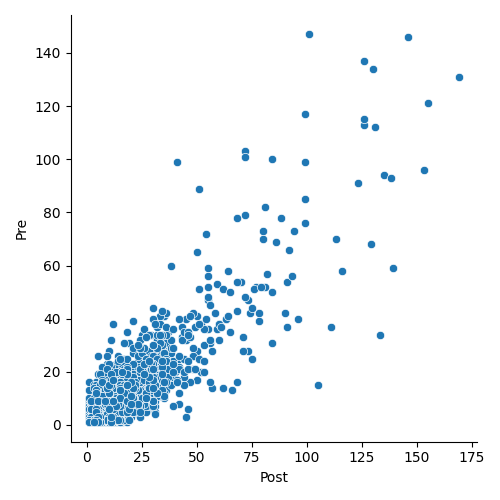
\includegraphics{plots/scattertext_sns.png}

\end{col}

\end{cols}
\end{frame}

\begin{frame}{Using colour}
\protect\hypertarget{using-colour}{}
Colour is another great way to convey information, and colorbrewer.org
tells you all about colour scales, of which there are three kinds:

\begin{itemize}
  \item<2->\textbf{Sequential} 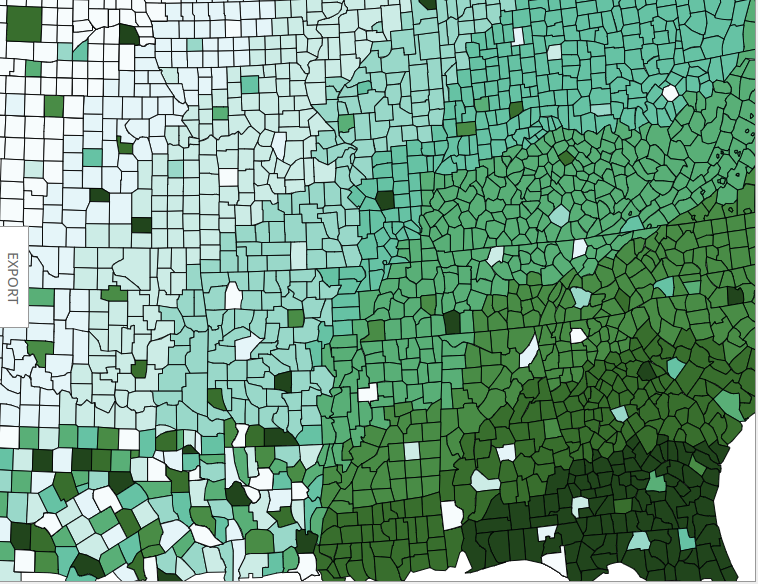
\includegraphics[height=1cm]{images/seq.png} colourscales show differences in magnitude of a continuous variable 
  \item<3->\textbf{Diverging} 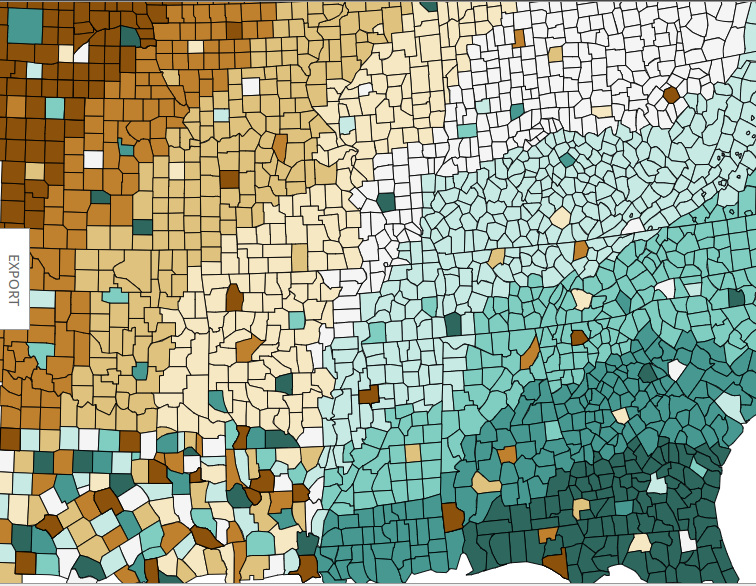
\includegraphics[height=1cm]{images/div.png} colourscales show \textit{symmetrical} differences in magnitude either side of a meaningful central point 
  \item<4->\textbf{Qualitative} 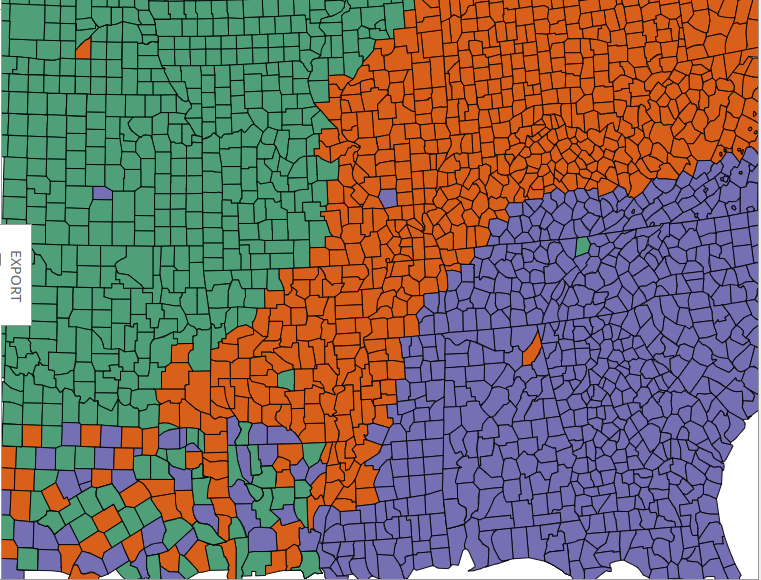
\includegraphics[height=1cm]{images/qual.png} colourscales shows different categories where there one category is neither greater than nor less than another 
\end{itemize}

\only<5>{PAY ATTENTION! to the colorblind-safe filter. A large proportion of people have reduced or no color discrimination along the red-green axis.}
\end{frame}

\begin{frame}[fragile]{Using colour II}
\protect\hypertarget{using-colour-ii}{}
\begin{cols}

\begin{col}{0.58\textwidth}

\scriptsize

\begin{Shaded}
\begin{Highlighting}[]
\NormalTok{ytfreq }\OtherTok{\textless{}{-}}\NormalTok{ dfmat }\SpecialCharTok{\%\textgreater{}\%} \FunctionTok{dfm\_weight}\NormalTok{(}\AttributeTok{scheme=}\StringTok{"prop"}\NormalTok{) }\SpecialCharTok{\%\textgreater{}\%} 
  \FunctionTok{textstat\_frequency}\NormalTok{(}\AttributeTok{groups=}\NormalTok{df}\SpecialCharTok{$}\NormalTok{era) }\SpecialCharTok{\%\textgreater{}\%}
  \FunctionTok{filter}\NormalTok{(docfreq}\SpecialCharTok{\textgreater{}}\DecValTok{10}\NormalTok{) }\SpecialCharTok{\%\textgreater{}\%}
  \FunctionTok{pivot\_wider}\NormalTok{(}
    \AttributeTok{id\_cols=}\NormalTok{feature, }
    \AttributeTok{names\_from=}\NormalTok{group, }
    \AttributeTok{values\_from=}\NormalTok{frequency}
\NormalTok{  )}

\NormalTok{ytfreq}\SpecialCharTok{$}\NormalTok{change }\OtherTok{\textless{}{-}} \FunctionTok{log}\NormalTok{(ytfreq}\SpecialCharTok{$}\NormalTok{Post }\SpecialCharTok{/}\NormalTok{ ytfreq}\SpecialCharTok{$}\NormalTok{Pre)}
\NormalTok{max\_change }\OtherTok{\textless{}{-}} \FunctionTok{max}\NormalTok{(}\FunctionTok{abs}\NormalTok{(ytfreq}\SpecialCharTok{$}\NormalTok{change), }\AttributeTok{na.rm=}\ConstantTok{TRUE}\NormalTok{)}

\NormalTok{p }\OtherTok{\textless{}{-}} \FunctionTok{ggplot}\NormalTok{(ytfreq, }\FunctionTok{aes}\NormalTok{(}\AttributeTok{x=}\NormalTok{Post, }\AttributeTok{y=}\NormalTok{Pre, }\AttributeTok{fill=}\NormalTok{change)) }\SpecialCharTok{+}
  \FunctionTok{geom\_point}\NormalTok{(}\AttributeTok{color=}\StringTok{"grey"}\NormalTok{, }\AttributeTok{shape=}\DecValTok{21}\NormalTok{) }\SpecialCharTok{+} 
  \FunctionTok{coord\_fixed}\NormalTok{() }\SpecialCharTok{+} 
  \FunctionTok{scale\_fill\_gradientn}\NormalTok{(}
    \AttributeTok{colors =} \FunctionTok{c}\NormalTok{(}\StringTok{"\#4575b4"}\NormalTok{,}\StringTok{"white"}\NormalTok{,}\StringTok{"\#d73027"}\NormalTok{),}
    \AttributeTok{values =}\NormalTok{ scales}\SpecialCharTok{::}\FunctionTok{rescale}\NormalTok{(}\FunctionTok{c}\NormalTok{(max\_change}\SpecialCharTok{*{-}}\DecValTok{1}\NormalTok{,}\DecValTok{0}\NormalTok{,max\_change)),}
    \AttributeTok{limits =} \FunctionTok{c}\NormalTok{(max\_change}\SpecialCharTok{*{-}}\DecValTok{1}\NormalTok{,max\_change)}
\NormalTok{  ) }\SpecialCharTok{+} 
  \FunctionTok{theme\_bw}\NormalTok{()}
\NormalTok{p}
\end{Highlighting}
\end{Shaded}

\begin{Shaded}
\begin{Highlighting}[]
\FunctionTok{ggsave}\NormalTok{(}\StringTok{"plots/scattertext\_gg\_2.png"}\NormalTok{, }\AttributeTok{width=}\DecValTok{4}\NormalTok{, }\AttributeTok{height=}\FloatTok{3.5}\NormalTok{)}
\end{Highlighting}
\end{Shaded}

\end{col}

\begin{col}{0.04\textwidth}
~

\end{col}

\begin{col}{0.38\textwidth}

\small

In this plot we get the \emph{proportion} of documents from each group
each term occurs in. We represent the \textbf{change} from one era to
another as a symmetrical variable either side of 0, and colour the
points on an appropriate \textbf{diverging} scale.

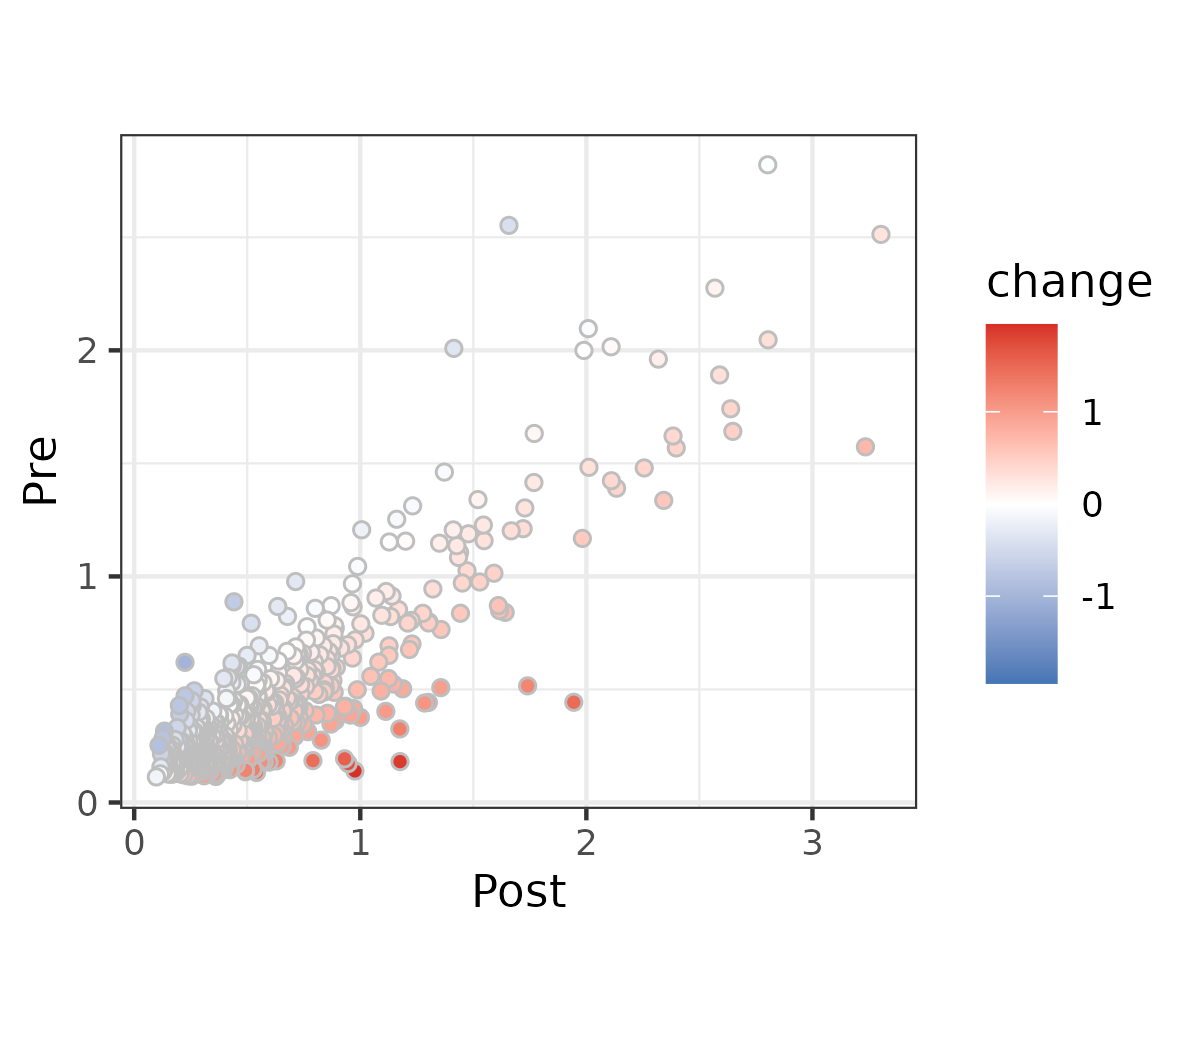
\includegraphics{plots/scattertext_gg_2.png}

\end{col}

\end{cols}
\end{frame}

\begin{frame}[fragile]{Adding labels}
\protect\hypertarget{adding-labels}{}
\begin{cols}

\begin{col}{0.58\textwidth}

\scriptsize

\begin{Shaded}
\begin{Highlighting}[]
\CommentTok{\#ytfreq \textless{}{-} ytfreq \textgreater{}max\_value \textless{}{-} max(ytfreq$Post\_2017, ytfreq$Pre\_2017)}
\NormalTok{labels }\OtherTok{\textless{}{-}}\NormalTok{ ytfreq }\SpecialCharTok{\%\textgreater{}\%} \FunctionTok{rowwise}\NormalTok{() }\SpecialCharTok{\%\textgreater{}\%} 
  \FunctionTok{mutate}\NormalTok{(}\AttributeTok{max\_value =} \FunctionTok{max}\NormalTok{(Post,Pre)) }\SpecialCharTok{\%\textgreater{}\%}
  \FunctionTok{filter}\NormalTok{(}
\NormalTok{    (}\FunctionTok{abs}\NormalTok{(change)}\SpecialCharTok{\textgreater{}}\FloatTok{0.4} \SpecialCharTok{\&}\NormalTok{ max\_value}\SpecialCharTok{\textgreater{}}\FloatTok{2.5}\NormalTok{)}
\NormalTok{  )}

\NormalTok{p }\SpecialCharTok{+} \FunctionTok{geom\_label}\NormalTok{(}\AttributeTok{data=}\NormalTok{labels, }\FunctionTok{aes}\NormalTok{(}\AttributeTok{label=}\NormalTok{feature))}
\end{Highlighting}
\end{Shaded}

\begin{Shaded}
\begin{Highlighting}[]
\FunctionTok{ggsave}\NormalTok{(}\StringTok{"plots/scattertext\_gg\_3.png"}\NormalTok{, }\AttributeTok{width=}\DecValTok{4}\NormalTok{, }\AttributeTok{height=}\FloatTok{3.5}\NormalTok{)}
\end{Highlighting}
\end{Shaded}

\end{col}

\begin{col}{0.04\textwidth}
~

\end{col}

\begin{col}{0.38\textwidth}
We can add labels so we know what the points represent, but these often
get in the way of readability

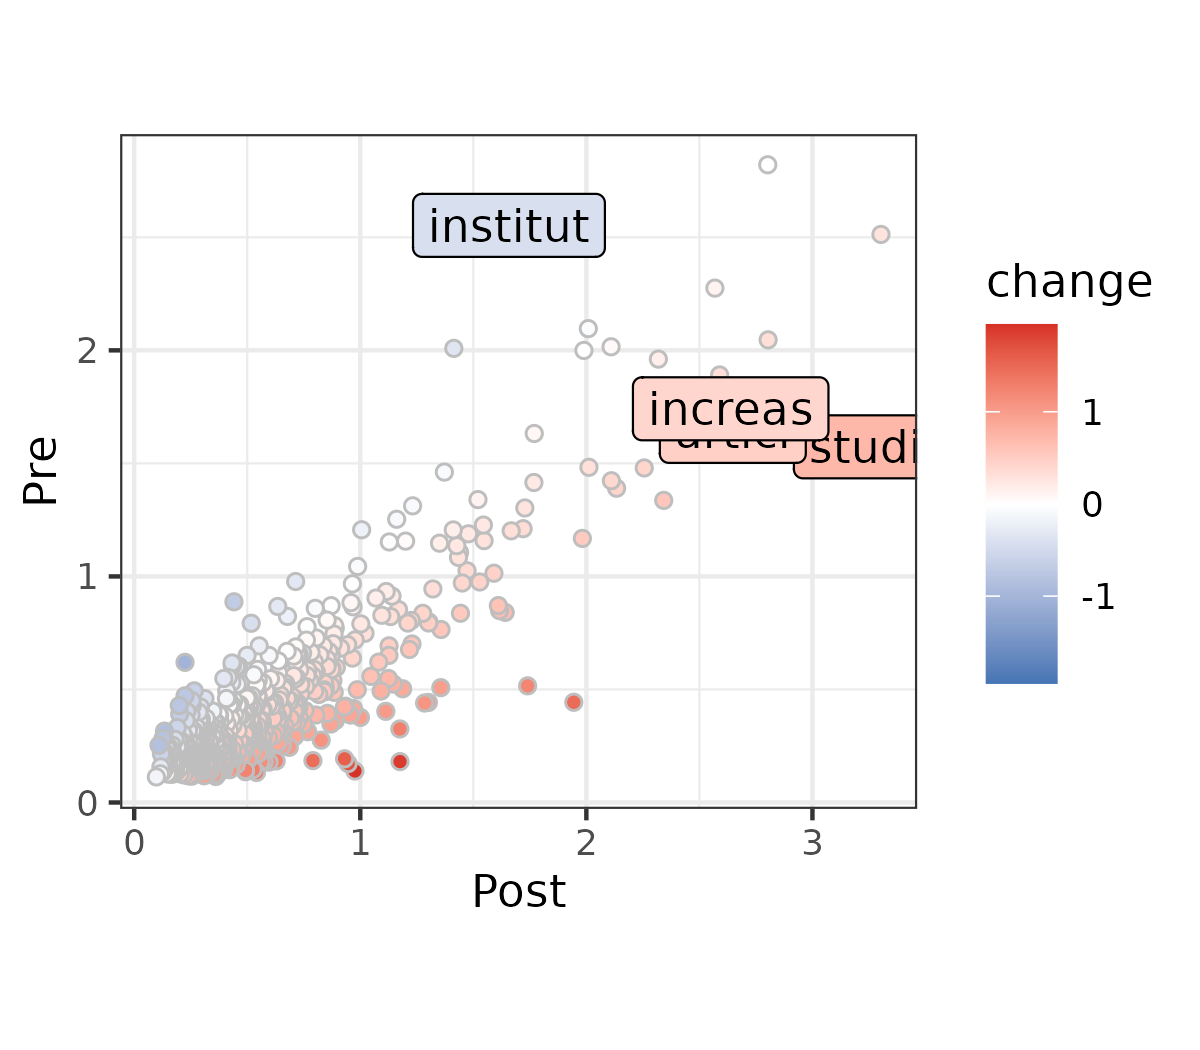
\includegraphics{plots/scattertext_gg_3.png}

\end{col}

\end{cols}
\end{frame}

\begin{frame}[fragile]{Adding labels with ggrepel}
\protect\hypertarget{adding-labels-with-ggrepel}{}
\begin{cols}

\begin{col}{0.58\textwidth}

\scriptsize

\begin{Shaded}
\begin{Highlighting}[]
\FunctionTok{library}\NormalTok{(ggrepel)}

\NormalTok{labels }\OtherTok{\textless{}{-}}\NormalTok{ ytfreq }\SpecialCharTok{\%\textgreater{}\%} \FunctionTok{rowwise}\NormalTok{() }\SpecialCharTok{\%\textgreater{}\%} 
  \FunctionTok{mutate}\NormalTok{(}\AttributeTok{max\_value =} \FunctionTok{max}\NormalTok{(Post,Pre)) }\SpecialCharTok{\%\textgreater{}\%}
  \FunctionTok{filter}\NormalTok{(}
\NormalTok{    (}\FunctionTok{abs}\NormalTok{(change)}\SpecialCharTok{\textgreater{}}\FloatTok{0.4} \SpecialCharTok{\&}\NormalTok{ max\_value}\SpecialCharTok{\textgreater{}}\FloatTok{2.5}\NormalTok{)}
\NormalTok{  )}

\NormalTok{p }\SpecialCharTok{+} \FunctionTok{geom\_label\_repel}\NormalTok{(}
  \AttributeTok{data=}\NormalTok{labels, }
  \FunctionTok{aes}\NormalTok{(}\AttributeTok{label=}\NormalTok{feature), }
  \AttributeTok{min.segment.length =} \DecValTok{0}
\NormalTok{)}
\end{Highlighting}
\end{Shaded}

\begin{Shaded}
\begin{Highlighting}[]
\FunctionTok{ggsave}\NormalTok{(}\StringTok{"plots/scattertext\_gg\_4.png"}\NormalTok{, }\AttributeTok{width=}\DecValTok{4}\NormalTok{, }\AttributeTok{height=}\FloatTok{3.5}\NormalTok{)}
\end{Highlighting}
\end{Shaded}

\end{col}

\begin{col}{0.04\textwidth}
~

\end{col}

\begin{col}{0.38\textwidth}
We can add labels so we know what the points represent, but these often
get in the way of readability

\medskip

\texttt{ggrepel} allows us to put labels in positions that maintain
readability

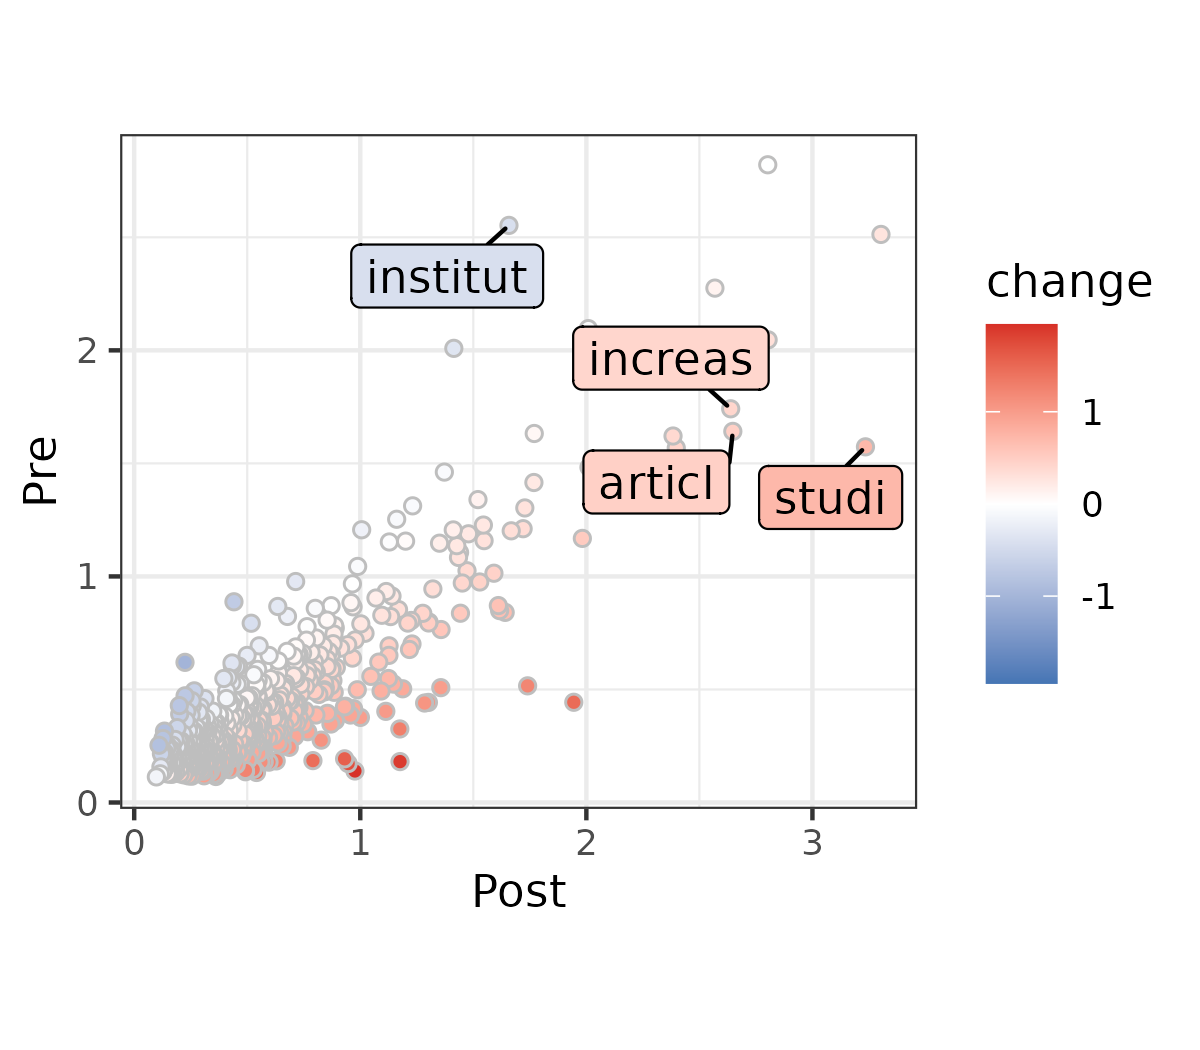
\includegraphics{plots/scattertext_gg_4.png}

\end{col}

\end{cols}
\end{frame}

\begin{frame}[fragile]{Color with Python}
\protect\hypertarget{color-with-python}{}
\begin{cols}

\begin{col}{0.58\textwidth}

\scriptsize

\begin{Shaded}
\begin{Highlighting}[]
\NormalTok{tidy\_dfm }\OperatorTok{=}\NormalTok{ pd.DataFrame()}
\ControlFlowTok{for}\NormalTok{ name, group }\KeywordTok{in}\NormalTok{ df.groupby(}\StringTok{"era"}\NormalTok{):}
\NormalTok{    counts }\OperatorTok{=}\NormalTok{ np.count\_nonzero(}
\NormalTok{      dfm[group.index,].A, axis}\OperatorTok{=}\DecValTok{0}
\NormalTok{    ) }\OperatorTok{/}\NormalTok{ group.shape[}\DecValTok{0}\NormalTok{]}
\NormalTok{    group\_df }\OperatorTok{=}\NormalTok{ pd.DataFrame(\{}
        \StringTok{"count"}\NormalTok{: counts,}
        \StringTok{"feature"}\NormalTok{: features,}
        \StringTok{"group"}\NormalTok{: name}
\NormalTok{    \})}
\NormalTok{    tidy\_dfm }\OperatorTok{=}\NormalTok{ pd.concat([}
\NormalTok{      tidy\_dfm, group\_df[group\_df[}\StringTok{"count"}\NormalTok{]}\OperatorTok{!=}\DecValTok{0}\NormalTok{]}
\NormalTok{    ]).reset\_index(drop}\OperatorTok{=}\VariableTok{True}\NormalTok{)}
\NormalTok{wide\_dfm }\OperatorTok{=}\NormalTok{ tidy\_dfm.pivot\_table(}
\NormalTok{  index}\OperatorTok{=}\StringTok{"feature"}\NormalTok{, columns}\OperatorTok{=}\StringTok{"group"}\NormalTok{, values}\OperatorTok{=}\StringTok{"count"}
\NormalTok{).reset\_index().reset\_index(drop}\OperatorTok{=}\VariableTok{True}\NormalTok{)}

\ImportTok{from}\NormalTok{ matplotlib.colors }\ImportTok{import}\NormalTok{ CenteredNorm}
\ImportTok{import}\NormalTok{ matplotlib.cm }\ImportTok{as}\NormalTok{ cm}
\NormalTok{colormap }\OperatorTok{=}\NormalTok{ cm.RdBu}
\NormalTok{norm }\OperatorTok{=}\NormalTok{ CenteredNorm()}
\NormalTok{wide\_dfm[}\StringTok{"change"}\NormalTok{] }\OperatorTok{=}\NormalTok{ np.log(wide\_dfm[}\StringTok{"Post"}\NormalTok{] }\OperatorTok{/}\NormalTok{ wide\_dfm[}\StringTok{"Pre"}\NormalTok{])}
\NormalTok{sns.relplot(}
\NormalTok{    data}\OperatorTok{=}\NormalTok{wide\_dfm, x}\OperatorTok{=}\StringTok{"Post"}\NormalTok{, y}\OperatorTok{=}\StringTok{"Pre"}\NormalTok{, hue}\OperatorTok{=}\StringTok{"change"}\NormalTok{, }
\NormalTok{    palette}\OperatorTok{=}\NormalTok{colormap, norm}\OperatorTok{=}\NormalTok{norm, edgecolor}\OperatorTok{=}\StringTok{"grey"}
\NormalTok{)}
\end{Highlighting}
\end{Shaded}

\begin{Shaded}
\begin{Highlighting}[]
\NormalTok{plt.savefig(}\StringTok{"plots/scattertext\_sns\_2.png"}\NormalTok{)}
\end{Highlighting}
\end{Shaded}

\end{col}

\begin{col}{0.04\textwidth}
~

\end{col}

\begin{col}{0.38\textwidth}
We can do the color rescaling much more easily with matplotlib (which we
use to tweak seaborn)

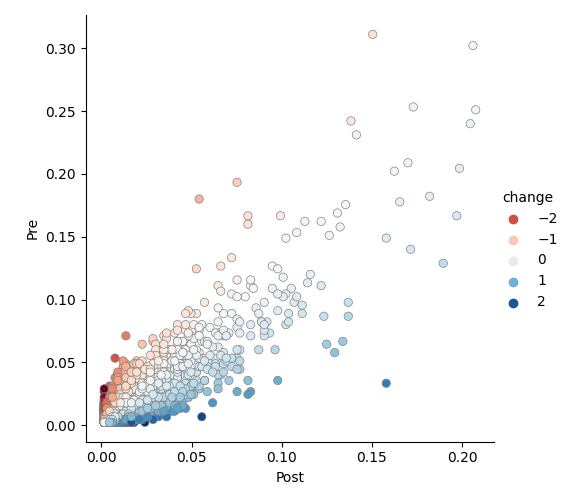
\includegraphics{plots/scattertext_sns_2.png}

\end{col}

\end{cols}
\end{frame}

\begin{frame}[fragile]{Color with Python}
\protect\hypertarget{color-with-python-1}{}
\begin{cols}

\begin{col}{0.58\textwidth}

\scriptsize

\begin{Shaded}
\begin{Highlighting}[]
\NormalTok{labels }\OperatorTok{=}\NormalTok{ wide\_dfm[}
\NormalTok{    (}\BuiltInTok{abs}\NormalTok{(wide\_dfm[}\StringTok{"change"}\NormalTok{])}\OperatorTok{\textgreater{}}\FloatTok{0.5}\NormalTok{) }\OperatorTok{\&}
\NormalTok{    (wide\_dfm[}\StringTok{"Post"}\NormalTok{]}\OperatorTok{+}\NormalTok{wide\_dfm[}\StringTok{"Pre"}\NormalTok{]}\OperatorTok{\textgreater{}}\FloatTok{.18}\NormalTok{)}
\NormalTok{]}

\ImportTok{from}\NormalTok{ adjustText }\ImportTok{import}\NormalTok{ adjust\_text}

\NormalTok{scatter }\OperatorTok{=}\NormalTok{ sns.relplot(}
\NormalTok{    data}\OperatorTok{=}\NormalTok{wide\_dfm, x}\OperatorTok{=}\StringTok{"Post"}\NormalTok{, y}\OperatorTok{=}\StringTok{"Pre"}\NormalTok{, hue}\OperatorTok{=}\StringTok{"change"}\NormalTok{, }
\NormalTok{    palette}\OperatorTok{=}\NormalTok{colormap, norm}\OperatorTok{=}\NormalTok{norm, edgecolor}\OperatorTok{=}\StringTok{"grey"}
\NormalTok{)}
\NormalTok{ax }\OperatorTok{=}\NormalTok{ scatter.ax}
\NormalTok{texts }\OperatorTok{=}\NormalTok{ []}
\ControlFlowTok{for}\NormalTok{ i, row }\KeywordTok{in}\NormalTok{ labels.iterrows():}
\NormalTok{    texts.append(ax.text(row[}\StringTok{"Post"}\NormalTok{], row[}\StringTok{"Pre"}\NormalTok{], row[}\StringTok{"feature"}\NormalTok{]))}

\NormalTok{adjust\_text(texts)}
\end{Highlighting}
\end{Shaded}

\begin{verbatim}
## 500
\end{verbatim}

\begin{Shaded}
\begin{Highlighting}[]
\NormalTok{plt.savefig(}\StringTok{"plots/scattertext\_sns\_3.png"}\NormalTok{)}
\end{Highlighting}
\end{Shaded}

\end{col}

\begin{col}{0.04\textwidth}
~

\end{col}

\begin{col}{0.38\textwidth}
We can do the color rescaling much more easily with matplotlib (which we
use to tweak seaborn)

To arrange text labels nicely we can use \texttt{adjustText}, which
works like ggrepel.

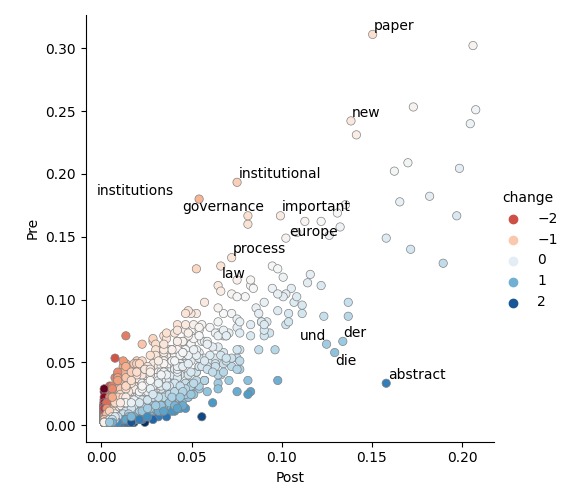
\includegraphics{plots/scattertext_sns_3.png}

\end{col}

\end{cols}
\end{frame}

\hypertarget{wrapup-and-outlook}{%
\section{Wrapup and outlook}\label{wrapup-and-outlook}}

\begin{frame}{Wrapup}
\protect\hypertarget{wrapup}{}
Today we strengthened our data our data management skills, and had a
refresher on ggplot2 / seaborn / matplotlib.

Getting data into the right format and plotting it is one of the
\emph{most import skills} as a data scientist!

The plotting libraries are much bigger than what we can cover, but you
have enough to get started and extend by \textbf{reading the
documentation}.
\end{frame}

\begin{frame}{Outlook}
\protect\hypertarget{outlook}{}
Next week we'll be getting more technical. We'll look at ways of
measuring similarity and at how we can do dimensionality reduction.
\end{frame}

\begin{frame}{Homework}
\protect\hypertarget{homework}{}
I will send you the homework assignment after class. This is due by
11:59 on 13 October.
\end{frame}

\begin{frame}[allowframebreaks]{}
  \bibliographytrue
  \bibliography{../presentation-resources/MyLibrary.bib}
\end{frame}

\end{document}
